\documentclass[11pt]{article}

\usepackage[margin=1in]{geometry}
\usepackage{amsmath,amssymb}
\usepackage{bm}
\usepackage{graphicx}
\usepackage{booktabs}
\usepackage{subcaption}
\usepackage{xcolor}
\usepackage{algorithm}
\usepackage{algpseudocode}
\usepackage[colorlinks=true,linkcolor=blue,citecolor=blue,urlcolor=blue]{hyperref}

% ---- notation --------------------------------------------------------- %
\newcommand{\vth}{\bm{\theta}}
\newcommand{\vthh}{\hat{\bm{\theta}}}
\newcommand{\vz}{\mathbf{z}}
\newcommand{\vu}{\mathbf{u}}
\newcommand{\vy}{\mathbf{y}}
\newcommand{\vF}{\mathbf{F}}
\newcommand{\vB}{\mathbf{B}}
\newcommand{\vD}{\mathbf{D}}
\newcommand{\vK}{\mathbf{K}}
\newcommand{\vM}{\mathbf{M}}
\newcommand{\vC}{\mathbf{C}}
\newcommand{\vN}{\mathbf{N}}
\newcommand{\vP}{\mathbf{P}}
\newcommand{\vQ}{\mathbf{Q}}
\newcommand{\vT}{\mathbf{T}}
\newcommand{\vL}{\mathbf{L}}
\newcommand{\vW}{\mathbf{W}}
\newcommand{\vA}{\mathbf{A}}
\newcommand{\vG}{\mathbf{G}}
\newcommand{\vx}{\mathbf{x}}
\newcommand{\vS}{\mathbf{S}}
\newcommand{\vPhi}{\hat{\bm{\Phi}}}
\newcommand{\vchi}{\hat{\bm{\chi}}}
\newcommand{\vpsi}{\bm{\psi}}
\newcommand{\rmd}{\,\mathrm{d}}
\newcommand{\ii}{\mathrm{i}}
\newcommand{\T}{^{\mathsf{T}}}
\newcommand{\HH}{^{\mathsf{H}}}
\newcommand{\half}{\tfrac12}
\newcommand{\Real}{\operatorname{Re}}
\newcommand{\Imag}{\operatorname{Im}}
\DeclareMathOperator{\softmax}{softmax}
\DeclareMathOperator{\softmin}{softmin}
\DeclareMathOperator{\relu}{relu}

\title{\bfseries Toolpath-Guided Anisotropy for Elastic Wave Control:\\
Theory and Algorithms for Orientation and Topology Optimization\\
of Continuous-Fiber Composites}
\author{}
\date{\today}

\begin{document}
\maketitle

\begin{abstract}
Continuous-fiber-reinforced polymer (CFRP) composites produced by additive
manufacturing admit spatially varying, curvilinear fiber layouts that endow the
material with a designable, locally anisotropic stiffness. This report gives a
complete and self-contained mathematical description of a density- and
orientation-based optimization framework for such composites, and of every
numerical routine in its implementation. We document (i) the finite-element
discretization and the \emph{exact} finite Fourier representation of the rotated
fiber stiffness that makes orientation-dependent assembly a scalar-weighted sum;
(ii) the compactly supported radial-basis-function (CS-RBF) orientation map and
its analytic spatial derivatives; (iii) the wave-projection ``toolpath
generation'' operator and its discrete adjoint; (iv) the quasi-static compliance
problem with local fiber-curvature (curl) constraints, reproducing Wong, Sanders
\& Rosen (\emph{Compos.\ Struct.}\ 2026); (v) the time-harmonic elastodynamic
solver with absorbing layers and the complex-symmetric adjoint used for
wave-energy localization, a multi-frequency (broadband) max--min objective, and
an elastic cloak; (vi) the Bloch band solver, Hellmann--Feynman eigenvalue
sensitivities, and the gauge-invariant Fukui--Hatsugai--Suzuki Berry-curvature
estimator; and (vii) the Method of Moving Asymptotes (MMA) and augmented-Lagrangian
optimizers, with explicit update formulas. Every sensitivity is derived by the
adjoint/Hellmann--Feynman method and verified against finite differences to
$\sim\!10^{-7}$. Numerical results demonstrate $>\!20\times$ single-frequency
energy focusing, uniform $\sim\!14\times$ broadband focusing, and $\sim\!15\times$
scattering reduction for a cloaked void, all driven purely by curved fiber
toolpaths in an otherwise homogeneous plate. Finally, using the same orientation
degree of freedom, we realize a \emph{topological} valley-Hall edge waveguide:
the rotation of a C$_3$ scatterer is a tunable Dirac mass whose sign sets the
valley Chern number, and a domain wall between mirror-partner orientations
guides a gap-traversing kink mode with a mid-gap/in-band transmission ratio of
$\sim\!10^3$. We further optimize the topological gap by MMA driven by
Hellmann--Feynman sensitivities over the density and fiber-orientation fields,
and give an honest accounting showing that in the anisotropic-fiber medium the
orientation is a necessary co-ingredient of the optimized gap, not a passive
accessory.
\end{abstract}

\tableofcontents

\section{Introduction}
Topology optimization of fiber-reinforced composites has classically produced a
density field together with a discrete fiber-orientation vector field, with the
continuous manufacturing toolpath generated only afterwards in
post-processing~\cite{wong2025,ren2024}. Because the as-manufactured
fiber--matrix distribution differs from the homogenized material assumed during
design, structural performance degrades in the transition to hardware. Recent
\emph{toolpath-integrated} formulations~\cite{wong2026,ren2024} close this gap by
generating an explicit fiber--matrix microstructure inside every optimization
iteration and by constraining fiber curvature so that the design is
manufacturable.

The same design freedom --- a smooth, curvilinear, locally anisotropic stiffness
tensor set by the fiber orientation --- is a powerful lever for \emph{elastic wave
control}: whereas the quasi-static problem steers load paths, its dynamic
counterpart steers energy paths. This document treats the density field $\vz$ and
the fiber-orientation field $\vth$ as design variables and changes only the
physics and objective between applications. The remainder is organized as a
reference: Part~I (\S\S2--6) develops the modeling primitives; Part~II
(\S\S7--12) the physics, objectives and their exact sensitivities; Part~III
(\S\S13--14) the optimization algorithms; Part~IV (\S15) the results; and \S16
records verification data.

Throughout, $N$ is the number of finite elements (and density variables), $M$ the
number of CS-RBF orientation support points, and $n_{\rm dof}$ the number of
displacement degrees of freedom. Element quantities carry a subscript $\ell$.

\part*{Part~I: Modeling primitives}

\section{Finite-element discretization}
The design domain is a rectangle $[0,L_x]\times[0,L_y]$ meshed by a regular grid
of $n_{\rm elx}\times n_{\rm ely}$ bilinear quadrilateral elements of size
$\Delta x\times\Delta y$. Each element $\ell$ has centroid $\mathbf{x}_\ell$
(a \emph{design point}) and area $A_\ell=\Delta x\,\Delta y$. In the vector
(in-plane) problem each node carries two displacement components; in the scalar
(antiplane-shear) problem, one.

\subsection{Shape functions and strain--displacement operator}
On the reference square $(\xi,\eta)\in[-1,1]^2$ the bilinear shape functions are
\begin{equation}
  N_1=\tfrac14(1-\xi)(1-\eta),\ N_2=\tfrac14(1+\xi)(1-\eta),\
  N_3=\tfrac14(1+\xi)(1+\eta),\ N_4=\tfrac14(1-\xi)(1+\eta).
\end{equation}
For an axis-aligned rectangle the Jacobian is constant,
$\mathbf{J}=\operatorname{diag}(\Delta x/2,\Delta y/2)$, $\det\mathbf{J}=
\tfrac14\Delta x\Delta y$, and physical gradients are
$\partial_x N_a=\tfrac{2}{\Delta x}\partial_\xi N_a$,
$\partial_y N_a=\tfrac{2}{\Delta y}\partial_\eta N_a$. The vector
strain--displacement matrix $\vB\in\mathbb{R}^{3\times8}$ (Voigt strains
$[\varepsilon_{xx},\varepsilon_{yy},\gamma_{xy}]$) has the standard block form
with $\vB_{0,2a}=\partial_xN_a$, $\vB_{1,2a+1}=\partial_yN_a$,
$\vB_{2,2a}=\partial_yN_a$, $\vB_{2,2a+1}=\partial_xN_a$. The scalar gradient
operator is $\vB^{s}=\mathbf{J}^{-1}[\partial_\xi\mathbf{N};\partial_\eta
\mathbf{N}]\in\mathbb{R}^{2\times4}$.

\subsection{Element matrices}
With a $2\times2$ Gauss rule (points $\pm1/\sqrt3$, unit weights) the element
stiffness for a constitutive matrix $\vD$, and the consistent mass, are
\begin{equation}
  \mathbf{k}(\vD)=\sum_{g}\vB(\xi_g,\eta_g)\T\,\vD\,\vB(\xi_g,\eta_g)\,\det\mathbf{J},
  \qquad
  \mathbf{m}(\rho)=\sum_{g}\rho\,\vN_g\T\vN_g\,\det\mathbf{J},
  \label{eq:elemmats}
\end{equation}
where $\vN$ collects the shape functions into the $2\times8$ (vector) or
$1\times4$ (scalar) interpolation matrix. Both maps are \emph{linear} in their
constitutive/density argument --- the property exploited in \S4. Global matrices
are assembled by scatter--add over the element-DOF map, precomputed once as
sparse row/column index arrays $(\mathbf{i}_K,\mathbf{j}_K)$.

\section{Anisotropic constitutive model}
\subsection{In-plane (vector) fiber and matrix}
In material axes the orthotropic fiber ply obeys plane-stress
$\vQ_f=\bigl[\begin{smallmatrix}Q_{11}&Q_{12}&0\\Q_{12}&Q_{22}&0\\0&0&Q_{66}
\end{smallmatrix}\bigr]$ with
\begin{equation}
  Q_{11}=\frac{E_{f1}}{1-\nu_{12}\nu_{21}},\quad
  Q_{12}=\frac{\nu_{12}E_{f2}}{1-\nu_{12}\nu_{21}},\quad
  Q_{22}=\frac{E_{f2}}{1-\nu_{12}\nu_{21}},\quad
  Q_{66}=G_{12},\quad \nu_{21}=\nu_{12}\tfrac{E_{f2}}{E_{f1}}.
\end{equation}
Rotating the ply to a physical angle $\theta$ uses the Voigt transformation
\begin{equation}
  \vT(\theta)=\begin{bmatrix}
  c^2 & s^2 & -2sc\\ s^2 & c^2 & 2sc\\ sc & -sc & c^2-s^2\end{bmatrix},
  \qquad c=\cos\theta,\ s=\sin\theta,
  \label{eq:Tmat}
\end{equation}
giving the rotated fiber stiffness $\vD_f(\theta)=\vT(\theta)\,\vQ_f\,
\vT(\theta)\T$. The isotropic polymer matrix has plane-stress stiffness
$\vD_m=\tfrac{E_m}{1-\nu_m^2}\bigl[\begin{smallmatrix}1&\nu_m&0\\\nu_m&1&0\\
0&0&(1-\nu_m)/2\end{smallmatrix}\bigr]$.

\subsection{Antiplane-shear (scalar) analogue}
For out-of-plane displacement $u_z(x,y)$ the governing operator is
$\nabla\!\cdot(\bm\mu(\theta)\nabla u_z)+\rho\omega^2u_z=0$ with a rank-2 shear
tensor
\begin{equation}
  \bm\mu(\theta)=\mathbf{R}(\theta)\operatorname{diag}(\mu_L,\mu_T)
  \mathbf{R}(\theta)\T
  = a\,\mathbf{I}+b\begin{bmatrix}\cos2\theta&\sin2\theta\\
  \sin2\theta&-\cos2\theta\end{bmatrix},\quad
  a=\tfrac{\mu_L+\mu_T}{2},\ b=\tfrac{\mu_L-\mu_T}{2},
  \label{eq:muscalar}
\end{equation}
where $\mathbf{R}(\theta)$ is the $2\times2$ rotation. The scalar element
stiffness is $\mathbf{k}^s(\bm\mu)=\sum_g(\vB^s)\T\bm\mu\,\vB^s\det\mathbf{J}$.

\section{Exact finite Fourier representation of orientation}
\label{sec:fourier}
Because $\vT(\theta)$ in \eqref{eq:Tmat} has entries that are degree-2 monomials
in $(c,s)$, each entry of $\vD_f(\theta)=\vT\vQ_f\vT\T$ is a trigonometric
polynomial of degree at most four, i.e.\ an exact linear combination of the five
basis functions
\begin{equation}
  \mathbf{c}(\theta)=\bigl[\,1,\ \cos2\theta,\ \sin2\theta,\ \cos4\theta,\
  \sin4\theta\,\bigr].
  \label{eq:fbasis}
\end{equation}
Since the element map \eqref{eq:elemmats} is linear in $\vD$, the element
stiffness inherits the \emph{exact} expansion
\begin{equation}
  \mathbf{k}_f(\theta)=\sum_{s=0}^{4}\mathbf{k}_{f,s}\,c_s(\theta),\qquad
  \mathbf{k}_{f,s}=\mathbf{k}\!\left(\mathbf{C}_s\right),
  \label{eq:kf}
\end{equation}
where $\mathbf{C}_s$ are the $3\times3$ coefficient matrices of $\vD_f$ in the
basis \eqref{eq:fbasis}. In the implementation the $\mathbf{C}_s$ are recovered by
an (overdetermined, exactly solvable) least-squares fit of $\vD_f(\theta)$
sampled densely over $\theta\in[-\pi,\pi)$; the residual is
$\mathcal{O}(10^{-16})$, confirming exactness. The four coefficient element
matrices $\mathbf{k}_{f,s}$ and the matrix-phase element stiffness
$\mathbf{k}_m=\mathbf{k}(\vD_m)$ are precomputed \emph{once}. During optimization,
assembly of $\mathbf{k}_f(\theta_\ell)$ and its derivative reduce to
\begin{equation}
  \mathbf{k}_f(\theta)=\sum_s\mathbf{k}_{f,s}c_s(\theta),\qquad
  \frac{\rmd\mathbf{k}_f}{\rmd\theta}=\sum_s\mathbf{k}_{f,s}\,c_s'(\theta),
  \label{eq:dkf}
\end{equation}
with $\mathbf{c}'(\theta)=[0,-2\sin2\theta,2\cos2\theta,-4\sin4\theta,
4\cos4\theta]$. The scalar case is the exact three-term analogue with basis
$\{1,\cos2\theta,\sin2\theta\}$ and closed-form coefficients $\mathbf{C}_0=a
\mathbf{I}$, $\mathbf{C}_1=b\operatorname{diag}(1,-1)$, $\mathbf{C}_2=b
\bigl[\begin{smallmatrix}0&1\\1&0\end{smallmatrix}\bigr]$ from
\eqref{eq:muscalar}. This precomputation is the key to making
orientation-dependent assembly (and its derivative) $\mathcal{O}(N)$ per
iteration.

\section{Density and orientation parametrization}
\subsection{Density: filter and SIMP}
The density variables $\vz\in[0,1]^N$ are regularized by a linear (cone) filter
$\vy=\vP\vz$, where
\begin{equation}
  P_{ij}=\frac{w_{ij}A_j}{\sum_k w_{ik}A_k},\qquad
  w_{ij}=\max\!\bigl(0,\,R-\lVert\mathbf{x}_i-\mathbf{x}_j\rVert\bigr),
  \label{eq:filter}
\end{equation}
with filter radius $R$. For periodic (tileable) unit cells the distance in
\eqref{eq:filter} is the minimum-image distance on the torus, so that the
physical density is seamlessly periodic. Intermediate densities are penalized by
the SIMP interpolation $E_\ell=\varepsilon+(1-\varepsilon)y_\ell^{\,p}$, with
penalty $p>1$ and Ersatz floor $\varepsilon$.

\subsection{Orientation: CS-RBF map and analytic spatial derivatives}
Orientation design variables $\vthh\in[-\tfrac\pi2,\tfrac\pi2]^M$ live at $M$
support points $\mathbf{x}_q$ and are interpolated to element angles
$\vth=\vPhi\,\vthh$ by normalized Wendland $C^2$ CS-RBFs
\begin{equation}
  \hat\Phi_{\ell q}=\frac{\phi_q(\mathbf{x}_\ell)}{\sum_{s}\phi_s(\mathbf{x}_\ell)},
  \qquad
  \phi_q(\mathbf{x})=(4r+1)\,[\max(0,1-r)]^4,\quad
  r=\frac{\sqrt{\lVert\mathbf{x}-\mathbf{x}_q\rVert^2+\varrho^2}}{r_s},
  \label{eq:csrbf}
\end{equation}
with support radius $r_s$ and a small $\varrho$ regularizing the spatial
derivative at $r\!\to\!0$. Normalization makes each row of $\vPhi$ sum to one, so
the bound $[-\tfrac\pi2,\tfrac\pi2]$ is preserved and $\vth$ is $C^1$. The
un-normalized radial derivative is
\begin{equation}
  \phi_{q,x}(\mathbf{x})=\frac{\partial\phi_q}{\partial x}
  =-\frac{20\,(x-x_q)}{r_s^2}\,[\max(0,1-r)]^3,
  \label{eq:phix}
\end{equation}
and likewise $\phi_{q,y}$; these follow from $\phi'(r)=-20\,r(1-r)^3$ and
$\partial r/\partial x=(x-x_q)/(r_s^2 r)$. The normalized derivative operators
follow from the quotient rule,
\begin{equation}
  \vPhi_{,x}=\vS^{-1}\bm\phi_{,x}-\operatorname{diag}(\vS_{,x})\,\vS^{-2}\bm\phi,
  \qquad
  \vS=\textstyle\sum_s\phi_s,\ \ \vS_{,x}=\sum_s\phi_{s,x},
  \label{eq:Phix}
\end{equation}
(with $\bm\phi$ the un-normalized CS-RBF matrix), and analogously $\vPhi_{,y}$.
These sparse $N\times M$ operators give the orientation-field spatial gradient
$\nabla\theta=(\vPhi_{,x}\vthh,\,\vPhi_{,y}\vthh)$ used by the curvature
constraint (\S9). Support-point discretizations are much coarser than the mesh
($M\ll N$).

\section{Wave-projection toolpath generation}
\label{sec:wave}
For the quasi-static CFRP problem the smooth orientation field is converted, in
each iteration, into an explicit fiber/matrix material state
$\vchi\in[0,1]^N$ ($1=$ fiber, $0=$ matrix) by the wave-projection analogy of
Rumpf \& Pazos and Ren et al.~\cite{ren2024}. A density-dependent spatial weight
$\alpha_\ell=H(z_\ell;\eta_\alpha,\beta)$ (smooth Heaviside, below) degrades the
phase reconstruction in void regions. The target phase gradient is
\begin{equation}
  \nabla\psi_\ell=\bigl(-\alpha_\ell\sin\theta_\ell,\ \alpha_\ell\cos\theta_\ell
  \bigr),
\end{equation}
i.e.\ $\nabla\psi\perp$ fibers. With centered finite-difference operators
$\vA_x,\vA_y$ (one-sided at boundaries), the phase is recovered in a
least-squares sense $\nabla\bm\psi\approx\vA\bm\psi$ via the normal equations
\begin{equation}
  \vG\bm\psi=\vA_x\T\mathbf{g}_x+\vA_y\T\mathbf{g}_y,\qquad
  \vG=\vA_x\T\vA_x+\vA_y\T\vA_y,
  \label{eq:phase}
\end{equation}
where $\vG$ is constant and prefactorized once (its single constant null vector
removed by pinning one anchor element, $\psi_{\rm anchor}=0$). A cosine wave of
wavelength $d$ and a second smooth Heaviside produce the towpreg and fiber states
\begin{equation}
  \chi_\ell=\half+\half\cos\!\Bigl(\tfrac{2\pi}{d}(\psi_\ell-\psi_0)\Bigr),\qquad
  \hat\chi_\ell=H(\chi_\ell;\eta,\beta),
  \label{eq:chi}
\end{equation}
where the smooth Heaviside and its derivative are
\begin{equation}
  H(x;\eta,\beta)=\frac{\tanh(\beta\eta)+\tanh\!\bigl(\beta(x-\eta)\bigr)}
  {\tanh(\beta\eta)+\tanh\!\bigl(\beta(1-\eta)\bigr)},\qquad
  H'(x)=\frac{\beta\bigl(1-\tanh^2\!\beta(x-\eta)\bigr)}
  {\tanh(\beta\eta)+\tanh\!\bigl(\beta(1-\eta)\bigr)}.
  \label{eq:heavi}
\end{equation}
The wavelength $d$ sets the towpreg width and $\eta$ the fiber volume fraction
within a towpreg, providing process-specific control (AFP vs.\ MEX).

\paragraph{Discrete adjoint.}
Given an upstream sensitivity $\partial f/\partial\hat\chi$, the chain rule
through \eqref{eq:chi}--\eqref{eq:phase} yields, with
$\partial\chi_\ell/\partial\psi_\ell=-\tfrac\pi d\sin(\tfrac{2\pi}{d}
(\psi_\ell-\psi_0))$,
\begin{equation}
  \bm\lambda_\psi=\vG^{-1}\!\Bigl(\tfrac{\partial f}{\partial\hat\chi}\odot
  H'(\bm\chi)\odot\tfrac{\partial\bm\chi}{\partial\bm\psi}\Bigr),\quad
  \mathbf{a}_x=\vA_x\bm\lambda_\psi,\ \ \mathbf{a}_y=\vA_y\bm\lambda_\psi,
  \label{eq:wpadj}
\end{equation}
(the pinned solve reuses the prefactorization of $\vG$), and finally
\begin{equation}
  \frac{\partial f}{\partial z_\ell}=\bigl(-a_{x,\ell}\sin\theta_\ell+
  a_{y,\ell}\cos\theta_\ell\bigr)\,H'(z_\ell),\qquad
  \frac{\partial f}{\partial\theta_\ell}=-\alpha_\ell\bigl(a_{x,\ell}
  \cos\theta_\ell+a_{y,\ell}\sin\theta_\ell\bigr).
  \label{eq:wpadj2}
\end{equation}
Equations \eqref{eq:wpadj}--\eqref{eq:wpadj2} were verified against finite
differences to $4$--$7$ digits.

\part*{Part~II: Physics, objectives, and sensitivities}

\section{Quasi-static compliance and its adjoint}
The global stiffness is assembled from the two-phase element matrices
\begin{equation}
  \vK(\vz,\vth)=\sum_{\ell}E_\ell\,\mathbf{k}^0_\ell,\qquad
  \mathbf{k}^0_\ell=\hat\chi_\ell\,\mathbf{k}_f(\theta_\ell)
  +(1-\hat\chi_\ell)\,\mathbf{k}_m,
\end{equation}
and the state solves $\vK\vu=\vF$; the objective is compliance $f=\vF\T\vu$,
which is self-adjoint, $\partial f/\partial s=-\vu\T(\partial\vK/\partial s)\vu$.
Collecting the element energy $e_\ell[\mathbf{k}]=\vu_\ell\T\mathbf{k}\,\vu_\ell$,
the full sensitivity chain is
\begin{align}
  \frac{\partial f}{\partial E_\ell}&=-e_\ell[\mathbf{k}^0_\ell],
  &\frac{\partial f}{\partial\vz}\Big|_{\rm SIMP}
  &=\vP\T\!\Bigl[\tfrac{\partial f}{\partial\mathbf E}\odot p(1-\varepsilon)
  \vy^{\,p-1}\Bigr],\\
  \frac{\partial f}{\partial\hat\chi_\ell}&=-E_\ell\,e_\ell[\mathbf{k}_f-
  \mathbf{k}_m], &(\text{then wave adjoint}~\eqref{eq:wpadj}\text{--}
  \eqref{eq:wpadj2})&\Rightarrow
  \tfrac{\partial f}{\partial\vz}\big|_{\chi},\ \tfrac{\partial f}
  {\partial\vth}\big|_{\chi},\\
  \frac{\partial f}{\partial\theta_\ell}\Big|_{\rm dir}
  &=-E_\ell\hat\chi_\ell\,e_\ell\!\left[\tfrac{\rmd\mathbf{k}_f}{\rmd\theta}
  \right], &\frac{\partial f}{\partial\vthh}
  &=\vPhi\T\Bigl(\tfrac{\partial f}{\partial\vth}\big|_{\rm dir}
  +\tfrac{\partial f}{\partial\vth}\big|_{\chi}\Bigr),
\end{align}
with $\partial f/\partial\vz=\partial f/\partial\vz|_{\rm SIMP}+\partial f/
\partial\vz|_\chi$. The derivative $\rmd\mathbf{k}_f/\rmd\theta$ comes for free
from \eqref{eq:dkf}.

\section{Volume constraints}
The composite- and fiber-volume constraints and their gradients are
\begin{equation}
  v_g=\frac{\sum_\ell A_\ell y_\ell}{\sum_\ell A_\ell}-v_{\rm all},\qquad
  v_{fg}=\frac{\sum_\ell A_\ell y_\ell\hat\chi_\ell}{\sum_\ell A_\ell}
  -v_{f,{\rm all}},
\end{equation}
$\partial v_g/\partial\vz=\vP\T(\mathbf A/\!\sum A)$, and for $v_{fg}$ the density
path $\partial v_{fg}/\partial\vy=\mathbf A\odot\vchi/\!\sum A$ plus the
material-state path $\partial v_{fg}/\partial\hat\chi=\mathbf A\odot\vy/\!\sum A$
routed through the wave adjoint to give $\partial v_{fg}/\partial\vz$ and
$\partial v_{fg}/\partial\vthh$.

\section{Fiber-curvature (curl) constraint}
Fiber-path curvature is limited by constraining the out-of-plane curl of the unit
orientation field $\mathbf v=(\cos\theta,\sin\theta)$:
\begin{equation}
  \zeta_\ell=\cos\theta_\ell\,(\vPhi_{,x}\vthh)_\ell
  +\sin\theta_\ell\,(\vPhi_{,y}\vthh)_\ell,\qquad
  \zeta_\ell^2\le\zeta_{\rm all}^2\quad(\ell=1,\dots,N).
  \label{eq:curl}
\end{equation}
Because $\theta=\vPhi\vthh$ is $C^1$, the Jacobian is analytic:
\begin{equation}
  \frac{\partial\zeta_\ell}{\partial\hat\theta_q}
  =\bigl(-\sin\theta_\ell\,a_\ell+\cos\theta_\ell\,b_\ell\bigr)\hat\Phi_{\ell q}
  +\cos\theta_\ell\,\hat\Phi_{,x,\ell q}+\sin\theta_\ell\,\hat\Phi_{,y,\ell q},
  \label{eq:curljac}
\end{equation}
with $a=\vPhi_{,x}\vthh$, $b=\vPhi_{,y}\vthh$. The $N$ local constraints are
handled by the augmented-Lagrangian scheme of \S14; \eqref{eq:curljac} was
verified to $\sim\!10^{-11}$.

\section{Time-harmonic elastodynamics}
For wave control the state at angular frequency $\omega$ solves the
complex-symmetric system
\begin{equation}
  \vD(\vth)\,\vu=\vF,\qquad
  \vD=(1+\ii\eta)\vK(\vth)-\omega^2\vM+\ii\,\omega\,\vC_{\rm sponge},
  \label{eq:D}
\end{equation}
with structural damping $\eta$, consistent mass $\vM$, and a mass-proportional
absorbing layer $\vC_{\rm sponge}=\sum_\ell c_\ell\,\mathbf{m}_\ell$. The
sponge coefficient ramps quadratically toward chosen open boundaries,
$c_\ell=c_0\,[\max(0,d_\ell)]^2$ with $d_\ell$ the normalized penetration into a
boundary margin, so that outgoing waves are attenuated before reflecting
(emulating an unbounded medium). For the pure wave-steering studies the density
is fixed solid ($\vz\equiv1$, $\vK=\sum_\ell\mathbf{k}_f(\theta_\ell)$), so
\emph{only} the fiber orientation is designed.

\subsection{Energy-localization objective and adjoint}
Let $\vL$ be a real diagonal operator selecting a focus region. The focus energy
$E=\vu\HH\vL\vu$ is real; differentiating $\vu=\vD^{-1}\vF$ and using
$\rmd\vu=-\vD^{-1}(\rmd\vD)\vu$ gives $\rmd E=-2\Real(\vu\HH\vL\vD^{-1}\rmd\vD\,
\vu)$. Introducing the adjoint field $\bm\lambda$ solving the conjugate system
(exploiting $\vD\T=\vD$, hence $\vD\HH=\overline{\vD}$),
\begin{equation}
  \overline{\vD}\,\bm\lambda=\vL\vu,\qquad
  \frac{\partial E}{\partial\theta_\ell}
  =-2\,\Real\!\Bigl[\bm\lambda_\ell\HH\,(1+\ii\eta)\,
  \frac{\rmd\mathbf{k}_f(\theta_\ell)}{\rmd\theta}\,\vu_\ell\Bigr],
  \label{eq:harmadj}
\end{equation}
since only $\vK$ (through $(1+\ii\eta)$) depends on $\theta$. The support-point
gradient is $\vPhi\T(\partial E/\partial\vth)$. Equation \eqref{eq:harmadj} was
verified to $\le\!10^{-7}$.

\subsection{Multi-frequency (broadband) max--min objective}
For frequencies $\{\omega_i\}_{i=1}^{n_f}$ with energies $E_i$ and straight-fiber
baselines $E_i^0$, define normalized gains $g_i=E_i/E_i^0$. A robust broadband
lens maximizes the worst-case gain through a Kreisselmeier--Steinhauser
soft-minimum
\begin{equation}
  \max_{\vth}\ \softmin_i(g_i),\qquad
  \softmin_i(g_i)=-\frac1\rho\ln\!\sum_i e^{-\rho g_i},\qquad
  w_i=\frac{e^{-\rho g_i}}{\sum_j e^{-\rho g_j}},
  \label{eq:softmin}
\end{equation}
whose gradient is the soft-min-weighted combination of single-frequency
gradients: $\partial_{\vth}\softmin=\sum_i w_i\,\partial_{\vth} g_i$. Each
$\partial_{\vth} E_i$ requires one forward solve \eqref{eq:D} and one adjoint solve
\eqref{eq:harmadj} at $\omega_i$. The alternative \texttt{sum} objective replaces
$w_i$ by unity. The soft-min form prevents starving one frequency to over-serve
another; \eqref{eq:softmin} was verified to $\le\!10^{-7}$ in both modes.

\subsection{Elastic cloaking objective}
For a plate containing a fixed void (a density hole, $z=0$ inside), the cloak
matches the field to a void-free reference $\vu_{\rm ref}$ in an observation
region $\vW$:
\begin{equation}
  J=(\vu-\vu_{\rm ref})\HH\vW(\vu-\vu_{\rm ref}),\qquad
  \overline{\vD}\,\bm\lambda=\vW(\vu-\vu_{\rm ref}),
\end{equation}
and $\partial J/\partial\theta_\ell$ has the identical form
\eqref{eq:harmadj} with $\vL\vu$ replaced by $\vW(\vu-\vu_{\rm ref})$; only the
fiber orientation in an annular shell around the void is designed. Verified to
$\sim\!10^{-8}$.

\section{Manufacturability constraints for wave-control toolpaths}
\label{sec:wavemfg}
The finite-domain devices of \S11 are, so far, purely academic: the fiber
orientation is free to vary at whatever rate the optimizer finds useful, with
no accounting for the fact that a real AFP or MEX head cannot lay a fiber tow
along an arbitrarily sharp turn, and no accounting for the mounting holes,
fasteners, or cut-outs that a real part carries. \texttt{wavetopo/wave\_mfg.py}
folds the two manufacturing constraints already developed for the
quasi-static problem (\S9) into the harmonic wave solver of \S11, so that
every wave-control device --- lens, broadband lens, and cloak --- can be
re-optimized under them without changing the underlying adjoint.

\subsection{True through-holes as a fixed two-phase field}
A drilled or printed-through hole is not a soft polymer inclusion; it is
\emph{air}. We therefore reuse the two-phase element interpolation of \S7 with
a fixed density field $\vz\in\{0,1\}^N$ (the hole geometry is given, not
designed) and an Ersatz stiffness floor $\varepsilon_v\ll1$ in place of a
matrix phase:
\begin{equation}
  \vK(\vth)=\sum_\ell s_\ell\,\mathbf{k}_f(\theta_\ell),\qquad
  s_\ell=\varepsilon_v+(1-\varepsilon_v)\,z_\ell^{\,p},\qquad
  \vM=\sum_\ell z_\ell\rho_f\,\mathbf{m}_\ell,
  \label{eq:holeK}
\end{equation}
i.e.\ the fiber composite is the \emph{only} material phase; the hole
contributes neither stiffness nor mass. Because \eqref{eq:holeK} is linear in
$\mathbf{k}_f(\theta_\ell)$, the harmonic adjoint \eqref{eq:harmadj} is
unchanged except for the constant per-element factor $s_\ell$ multiplying
$(1+\ii\eta)\,\rmd\mathbf{k}_f/\rmd\theta$ --- the fiber orientation is only
ever designed (and only ever contributes gradient) where material actually
exists. The same construction gives a \emph{broadband, multi-hole} cloak: for
frequencies $\{\omega_i\}$ with reference fields $\vu_{{\rm ref},i}$ (solved
on the hole-free plate) and observation weights $\vW$, the worst-case
mismatch objective is the direct analogue of \eqref{eq:softmin},
\begin{equation}
  \min_{\vth}\ \softmax_i\bigl(J_i/J_i^0\bigr),\qquad
  J_i=(\vu_i-\vu_{{\rm ref},i})\HH\vW(\vu_i-\vu_{{\rm ref},i}),\qquad
  \softmax_\rho(v)=\tfrac1\rho\ln\textstyle\sum_ie^{\rho v_i},
  \label{eq:softmax_cloak}
\end{equation}
normalizing by the uncloaked (straight-fiber) mismatch $J_i^0$ at each
frequency, with gradient the KS-weighted combination of the per-frequency
adjoints \eqref{eq:harmadj}, exactly as in \S11.2.

\subsection{Fiber-curvature (curl) limits in the wave problem}
The orientation field $\theta=\vPhi\vthh$ is the same $C^1$ CS-RBF map used in
the quasi-static problem, so the curl (fiber-curvature) constraint
\eqref{eq:curl}--\eqref{eq:curljac} applies unchanged: $\zeta_\ell=\cos
\theta_\ell(\vPhi_{,x}\vthh)_\ell+\sin\theta_\ell(\vPhi_{,y}\vthh)_\ell$, with
the local limit $\zeta_\ell^2\le\zeta_{\rm all}^2$ enforced only over solid
(non-hole) elements, $\{\ell: z_\ell>\tfrac12\}$. We reuse the
augmented-Lagrangian driver of \S14 verbatim (objective $J$ from
\S11.1--11.3 or \S16.1 replacing compliance $f$; constraints normalized as
$g_\ell=\zeta_\ell^2/\zeta_{\rm all}^2-1$ so the penalty scale is
frequency/objective-independent), with one addition: because a harmonic
objective's response to $\theta$ is oscillatory (through $\cos,\sin$ in
$\vD$) rather than monotone as in compliance, the coupled MMA/AL subproblem
can \emph{overshoot} the curl boundary by a few percent even after the
penalty $\mu$ saturates at $\mu_{\max}$. We therefore add a cheap bisection
correction: at each outer iterate that is near-feasible
($\max_\ell|\zeta_\ell|/\zeta_{\rm all}<1.25$), scale the orientation
solution toward straight fibers, $\vthh_\kappa=\kappa\vthh$, and bisect
$\kappa\in(0,1]$ (using only curl evaluations, no re-solve of the wave
equation) for the largest $\kappa$ with $\max_\ell|\zeta_\ell(\kappa\vthh)|
\le\zeta_{\rm all}$; because $\zeta(\mathbf 0)=0$, feasibility at $\kappa=0$
is guaranteed and the bisection always succeeds. The resulting exactly
feasible design is scored by the true objective and kept if it improves on
the best feasible iterate so far. This costs $O(40)$ sparse mat-vecs per
outer iteration (curl only) and no additional wave solves.

\subsection{Verification}
All adjoints in \texttt{wave\_mfg.py} --- the through-hole-scaled focus
gradient, the broadband match gradient (sum and soft-max modes), and the
curl Jacobian --- were verified against central finite differences to
$\lesssim\!10^{-6}$ (Table~\ref{tab:verify}, rows added in
\texttt{tests/test\_wave\_mfg.py}); the augmented-Lagrangian driver was
checked to return a design satisfying the curl limit to within the tolerance
$\text{tolC}=5\times10^{-3}$ on the problems of \S16.5.

\section{Periodic (Bloch) analysis}
\subsection{Bloch reduction and the generalized eigenproblem}
For a wavevector $\mathbf k$ the displacement obeys $\vu(\mathbf x+\mathbf a)=
e^{\ii\mathbf k\cdot\mathbf a}\vu(\mathbf x)$. Assembling $\vK,\vM$ on the open
cell and imposing periodicity by a complex reduction matrix $\vT(\mathbf k)$
(each boundary node slaved to its interior master with phase $e^{\ii\mathbf k
\cdot\mathbf a}$) yields the Hermitian generalized eigenproblem
\begin{equation}
  \vK_r(\mathbf k)\bm\varphi=\omega^2\vM_r(\mathbf k)\bm\varphi,\qquad
  \vK_r=\vT\HH\vK\vT,\ \ \vM_r=\vT\HH\vM\vT.
  \label{eq:bloch}
\end{equation}
Lowest bands use a dense Hermitian solver; a few interior bands near a target
$\sigma=\omega_\star^2$ use sparse shift-invert (Lanczos), with the eigenvectors
re-normalized to $\bm\varphi\HH\vM_r\bm\varphi=1$ (giving $\sim\!10\times$
speedup for the valley studies). The two-phase cell interpolates
$\mathbf{k}^0_\ell=z_\ell^p\mathbf{k}_f(\theta_\ell)+(1-z_\ell^p)\mathbf{k}_m$ and
$\rho_\ell=z_\ell\rho_f+(1-z_\ell)\rho_m$.

\subsection{Eigenvalue sensitivities (Hellmann--Feynman)}
For a simple eigenvalue $\lambda=\omega^2$ with $\vM_r$-normalized $\bm\varphi$
and full-space vector $\bm\phi=\vT\bm\varphi$ (with $\vT$ design-independent),
\begin{equation}
  \frac{\partial\lambda}{\partial z_\ell}
  =p\,z_\ell^{p-1}\,\bm\phi_\ell\HH(\mathbf{k}_f-\mathbf{k}_m)\bm\phi_\ell
  -\lambda\,(\rho_f-\rho_m)\,\bm\phi_\ell\HH\mathbf{m}_\ell\bm\phi_\ell,\qquad
  \frac{\partial\lambda}{\partial\theta_\ell}
  =z_\ell^p\,\bm\phi_\ell\HH\frac{\rmd\mathbf{k}_f}{\rmd\theta}\bm\phi_\ell,
  \label{eq:hf}
\end{equation}
and $\partial\omega/\partial(\cdot)=\partial\lambda/\partial(\cdot)/(2\omega)$,
with the support-point orientation gradient $\vPhi\T(\partial\lambda/\partial
\vth)$. Verified to $\sim\!10^{-6}$ across bands.

\subsection{Berry curvature: Fukui--Hatsugai--Suzuki}
For an isolated band we compute the (gauge-invariant) discrete Berry curvature on
an $n_k\times n_k$ grid over the Brillouin zone. Using the $\vM$-weighted inner
product of full-space Bloch states $\bm\phi(\mathbf k)=\vT(\mathbf k)\bm\varphi
(\mathbf k)$, form directed link variables and plaquette field strength
\begin{equation}
  U_\mu(\mathbf k)=\langle\bm\phi(\mathbf k)|\vM|\bm\phi(\mathbf k+\mathbf e_\mu)
  \rangle,\qquad
  F(\mathbf k)=\Imag\ln\!\bigl[U_x(\mathbf k)U_y(\mathbf k{+}\mathbf e_x)
  U_x(\mathbf k{+}\mathbf e_y)^{*}U_y(\mathbf k)^{*}\bigr].
  \label{eq:fhs}
\end{equation}
Any $\mathbf k$-local phase of $\bm\phi$ cancels around the loop, so $F$ is
gauge invariant. The Chern number is $C=\tfrac1{2\pi}\sum_{\mathbf k}F$ and the
\emph{valley} Chern is the half-Brillouin-zone sum about $K$ or $K'$. The
estimator was validated on the Qi--Wu--Zhang model, recovering the exact
$C\in\{0,\pm1\}$ across its phase transitions.

\subsection{Band-gap objectives}
Directional and complete gaps between bands $p,p{+}1$ over a $\mathbf k$-sample
$\mathcal S$ use smooth KS aggregation
\begin{equation}
  \text{gap}=\softmin_{\mathbf k\in\mathcal S}\omega_{p+1}(\mathbf k)
  -\softmax_{\mathbf k\in\mathcal S}\omega_{p}(\mathbf k),\qquad
  \softmax_\rho(v)=\tfrac1\rho\ln\!\sum e^{\rho v},
\end{equation}
with gradients the KS-weighted eigenvalue sensitivities \eqref{eq:hf}. The
directional band-gap optimizer adds an orthogonal-direction penalty
$\relu(\text{gap}_\perp)$ to keep the gap direction-selective; the valley-gap
optimizer adds an isolation penalty $\relu(m-(\omega_p-\omega_{p-1}))+\relu(m-
(\omega_{p+2}-\omega_{p+1}))$ to keep the Dirac pair isolated; both add a volume
penalty $c(\text{vol}-\text{vol}_\star)^2$.

\part*{Part~III: Optimization algorithms}

\section{Method of Moving Asymptotes (bound-constrained)}
All problems here fold their constraints into the objective (augmented Lagrangian
or explicit penalties), so we use MMA with $m=0$ explicit constraints, whose
separable convex subproblem has a closed-form primal solution. At design $\vx$
with objective gradient $\partial_x f_0$, MMA maintains moving asymptotes
$\mathbf L,\mathbf U$ that bracket $\vx$. On iteration $t$:

\begin{algorithm}[h]
\caption{MMA update (\texttt{MMA.update})}
\begin{algorithmic}[1]
\State \textbf{asymptotes:} if $t\le2$: $\mathbf L=\vx-s_0\,\mathbf{span}$,
  $\mathbf U=\vx+s_0\,\mathbf{span}$; \; else
  $\bm\gamma=\{1.2,\,0.7,\,1\}$ by $\operatorname{sign}\!\bigl[(\vx-\vx^{-1})
  \odot(\vx^{-1}-\vx^{-2})\bigr]$,
\Statex \hspace{1.2em}$\mathbf L=\vx-\bm\gamma\odot(\vx^{-1}-\mathbf L^{-1})$,\;
  $\mathbf U=\vx+\bm\gamma\odot(\mathbf U^{-1}-\vx^{-1})$, then clip to
  $[\vx-10\,\mathbf{span},\vx-0.01\,\mathbf{span}]$ etc.
\State \textbf{move limits:} $\bm\alpha=\max(\vx_{\min},\mathbf L+0.1(\vx-\mathbf
  L),\vx-\text{mv}\,\mathbf{span})$, \;
  $\bm\beta=\min(\vx_{\max},\mathbf U-0.1(\mathbf U-\vx),\vx+\text{mv}\,
  \mathbf{span})$
\State \textbf{convex coefficients:} with
  $\partial_x f^\pm=\max(\pm\partial_x f_0,0)$ and $r=r_0/\mathbf{span}$,
\Statex \hspace{1.2em}$\mathbf p_0=(\mathbf U-\vx)^2(1.001\,\partial_xf^{+}
  +0.001\,\partial_xf^{-}+r)$,\;
  $\mathbf q_0=(\vx-\mathbf L)^2(0.001\,\partial_xf^{+}+1.001\,\partial_xf^{-}+r)$
\State \textbf{closed-form minimizer:}
  $\displaystyle \vx^{\rm new}=\frac{\sqrt{\mathbf p_0}\odot\mathbf L
  +\sqrt{\mathbf q_0}\odot\mathbf U}{\sqrt{\mathbf p_0}+\sqrt{\mathbf q_0}}$,
  then clip to $[\bm\alpha,\bm\beta]$
\end{algorithmic}
\end{algorithm}

The step-4 formula is the exact stationary point of the separable MMA
approximation $\sum_j\bigl[p_{0j}/(U_j-x_j)+q_{0j}/(x_j-L_j)\bigr]$, obtained by
setting each coordinate derivative to zero. The small mixing ($0.001$) and
$r_0$ regularization keep $\mathbf p_0,\mathbf q_0>0$.

\section{Augmented Lagrangian for local constraints}
For the many local curl constraints, the outer loop solves a sequence of
bound-constrained subproblems (each \texttt{MMAIter} MMA steps) with the
augmented-Lagrangian objective
\begin{equation}
  \mathcal L=f+\underbrace{\sum_{j\in\text{global}}\!\Bigl[\lambda_j h_j
  +\tfrac\mu2 h_j^2\Bigr]
  +\frac1N\!\sum_{j\in\text{local}}\!\Bigl[\lambda_j h_j+\tfrac\mu2 h_j^2\Bigr]}
  _{J},\qquad
  h_j=\max\!\Bigl(g_j,\,-\tfrac{\lambda_j}{\mu}\Bigr),
  \label{eq:al}
\end{equation}
where the $1/N$ scaling makes the local-constraint penalty independent of mesh
size. Its gradient is
$\partial_{\vW}\mathcal L=\partial_{\vW} f+\sum_j(\lambda_j+\mu h_j)\,\partial_{\vW} g_j
\,\mathbf 1[g_j>-\lambda_j/\mu]$, with $\partial_{\vW} g_j$ the volume/curl
gradients of \S8--9. After each subproblem the multipliers and penalty update as
$\lambda_j\leftarrow\max(\lambda_j+\mu h_j,0)$ and $\mu\leftarrow\min(\xi\mu,
\mu_{\max})$.

\begin{algorithm}[h]
\caption{Augmented-Lagrangian driver (\texttt{optimize\_cfrp})}
\begin{algorithmic}[1]
\State init $\vz,\vthh$; $\bm\lambda\!=\!\lambda_0$; $\mu\!=\!\mu_0$;
  $\text{best}\!=\!\infty$
\For{$k=0,\dots,\text{MaxOuter}$}
  \For{$\text{MMAIter}$ steps} \Comment{inner: minimize $\mathcal L$}
    \State toolpath generation (wave projection \eqref{eq:chi}); solve
      $\vK\vu=\vF$; evaluate $f,\mathbf g,\bm\zeta$
    \State $\vW\gets\textsc{MMA.update}(\vW,\partial_{\vW}\mathcal L)$
  \EndFor
  \State evaluate feasibility (volume, $\max|\zeta|/\zeta_{\rm all}$); if
    feasible and $f<\text{best}$, store best
  \State $\lambda_j\gets\max(\lambda_j+\mu h_j,0)$;\;
    \textbf{if} infeasible \textbf{then} $\mu\gets\min(\xi\mu,\mu_{\max})$
    \Comment{gate penalty growth}
  \State \textbf{if} $\Delta\vW<\text{tolD}$ and curl feasible \textbf{then
    break}; \textbf{if} stale \textbf{then break}
\EndFor
\State \Return best feasible design
\end{algorithmic}
\end{algorithm}

Two safeguards are essential in practice and are highlighted in Algorithm~2.
First, the penalty $\mu$ is grown \emph{only while a constraint is violated};
continuing to inflate $\mu$ after feasibility ill-conditions the MMA subproblem
and destabilizes an already-converged design. Second, the driver returns the best
\emph{feasible} iterate rather than the last, since MMA on the coupled
density--orientation problem oscillates at the few-percent level rather than
reaching a tight design-change tolerance.

\part*{Part~IV: Results}

\section{Numerical results}
\subsection{Validation: curvature-constrained CFRP cantilever}
We reproduce the no-void cantilever of Wong et al.~\cite{wong2026} at their
$240\times150$ resolution (Table~\ref{tab:cant}). Without a curl constraint the
optimizer recovers a two-strut design; imposing $\zeta_{\rm all}=2\,\mathrm{m}^{-1}$
drives the maximum fiber curvature to the allowable limit at a compliance cost,
matching the reported behavior. Figure~\ref{fig:cant} shows the clean
(filtered/projected) topologies, fiber streamlines, explicit towpregs, and curl
maps.

\begin{table}[h]
\centering
\caption{No-void cantilever: present results vs.\ Wong et al.~\cite{wong2026}.}
\label{tab:cant}
\begin{tabular}{lcccc}
\toprule
& $f$ (ours) & $f$ (paper) & $|\zeta|_{\max}$ ours & $|\zeta|_{\max}$ paper\\
\midrule
no curl constraint & 0.452 & 0.42 & 10.7 & 8.04\\
curl $\le2\,\mathrm{m}^{-1}$ & 0.577 & 0.49 & 1.93 & 2.00\\
\bottomrule
\end{tabular}
\end{table}

\begin{figure}[h]
\centering
\begin{subfigure}{0.49\textwidth}
  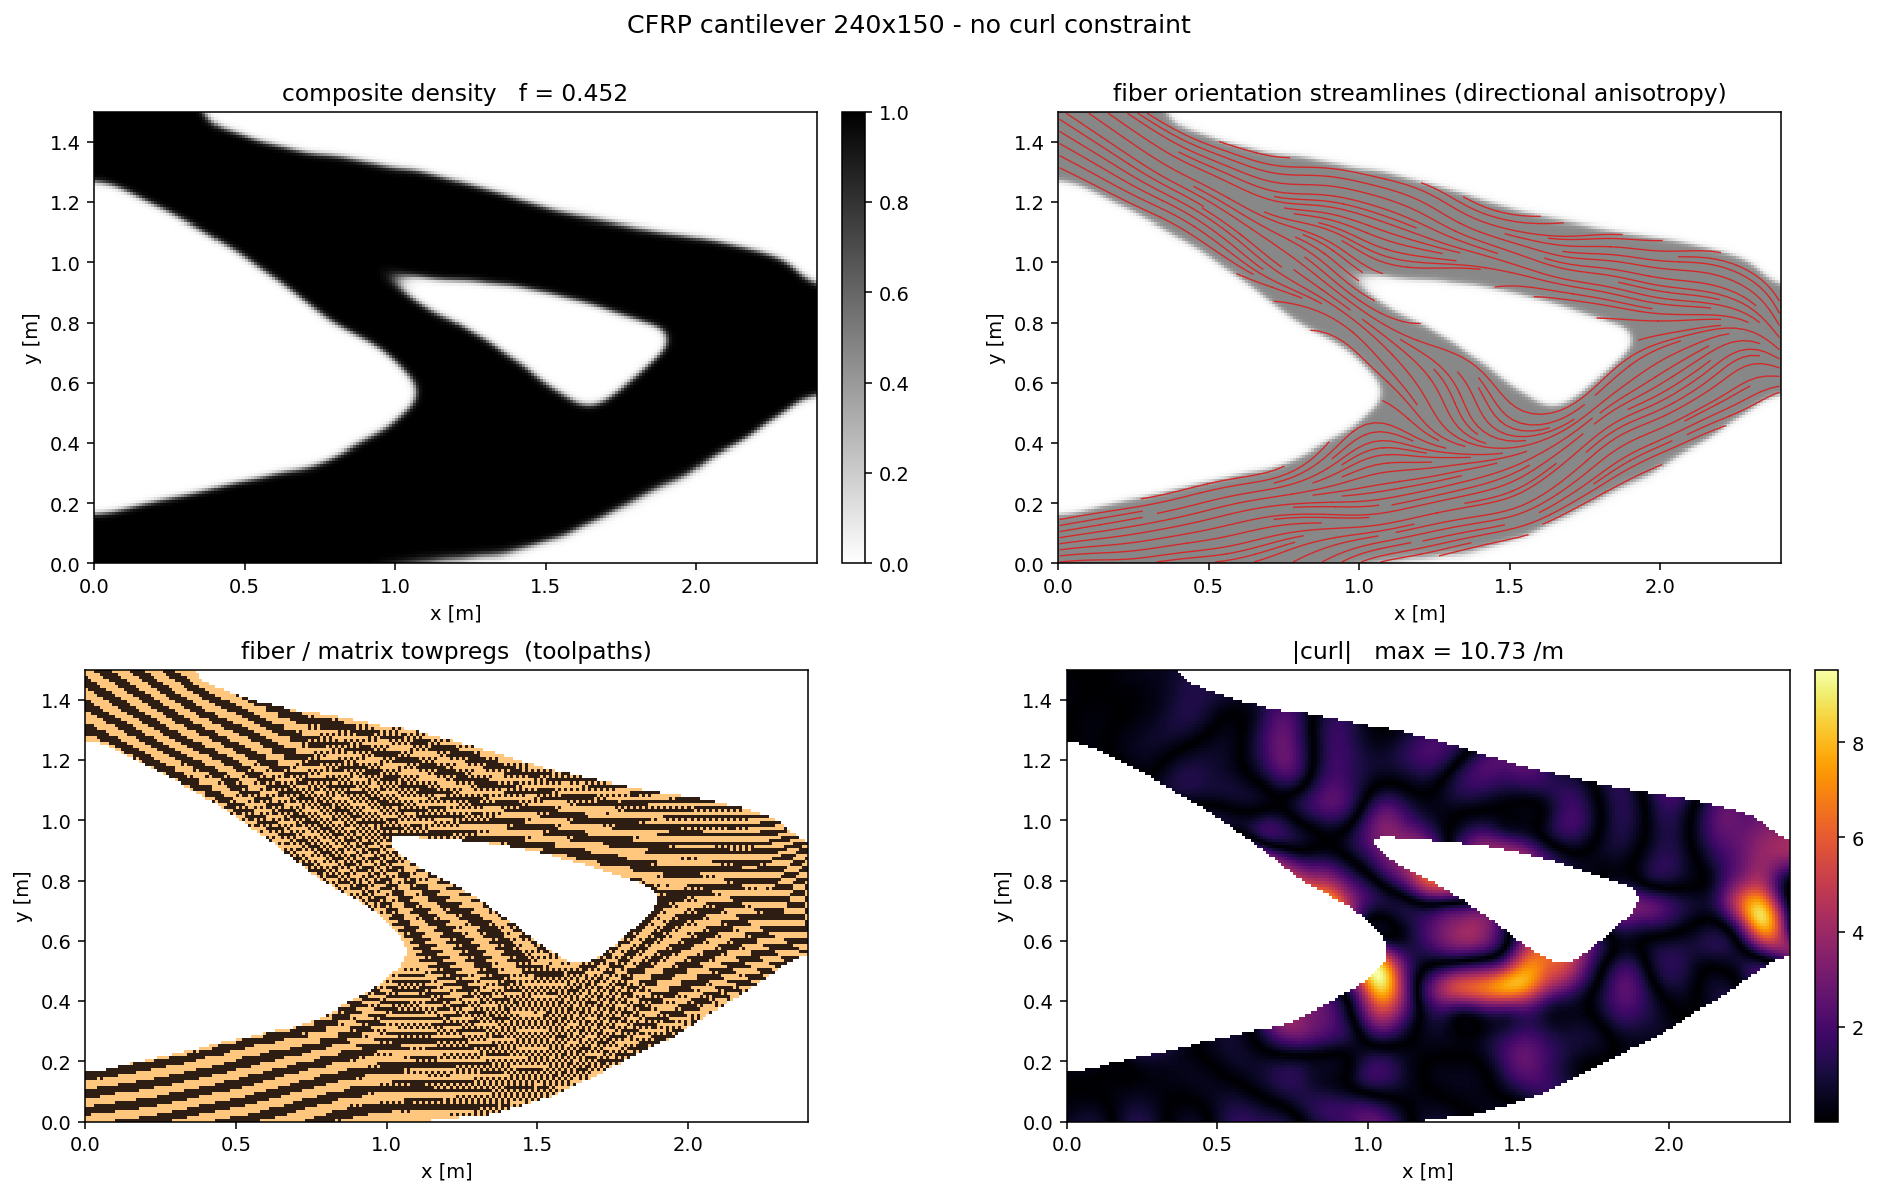
\includegraphics[width=\linewidth]{figs/cant_nocurl.png}
  \caption{no curl constraint}
\end{subfigure}
\begin{subfigure}{0.49\textwidth}
  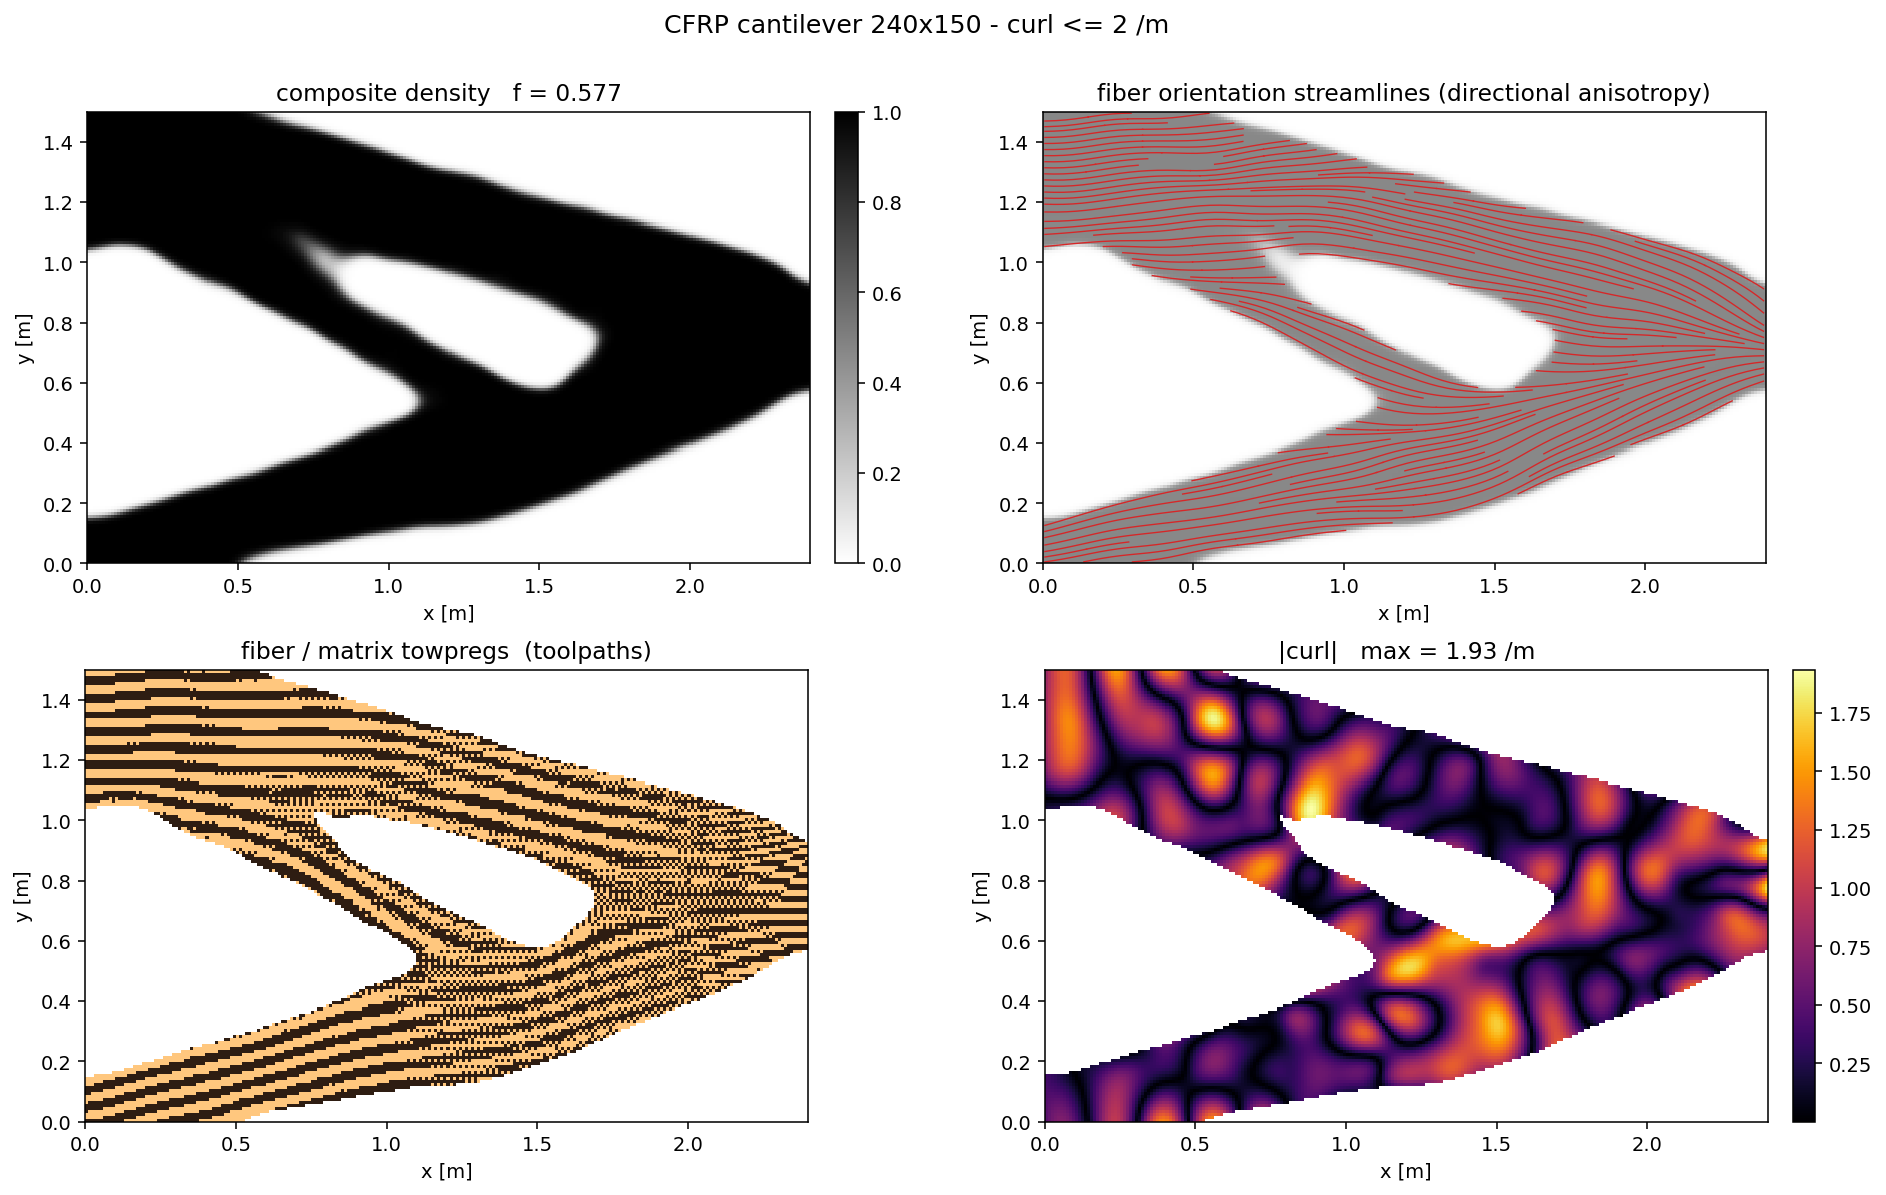
\includegraphics[width=\linewidth]{figs/cant_curl2.png}
  \caption{$\zeta_{\rm all}=2\,\mathrm{m}^{-1}$}
\end{subfigure}
\caption{Curvature-constrained CFRP cantilever (density, fiber streamlines,
fiber/matrix toolpaths, and $|\zeta|$ map). The curl constraint removes the
high-curvature hot spots and enlarges the load-path turning radii.}
\label{fig:cant}
\end{figure}

\subsection{Wave-energy localization (single frequency)}
A solid composite plate is driven by a plane pressure wave from the left edge;
only the fiber orientation is optimized to maximize elastic energy in a small box
on the right. The optimized fibers curve into a converging lens and concentrate
the field at the target with a $\mathbf{20.6\times}$ energy gain over the
straight-fiber baseline (Figure~\ref{fig:lens}). The material is homogeneous
everywhere --- only the fiber \emph{direction} varies.

\begin{figure}[h]
\centering
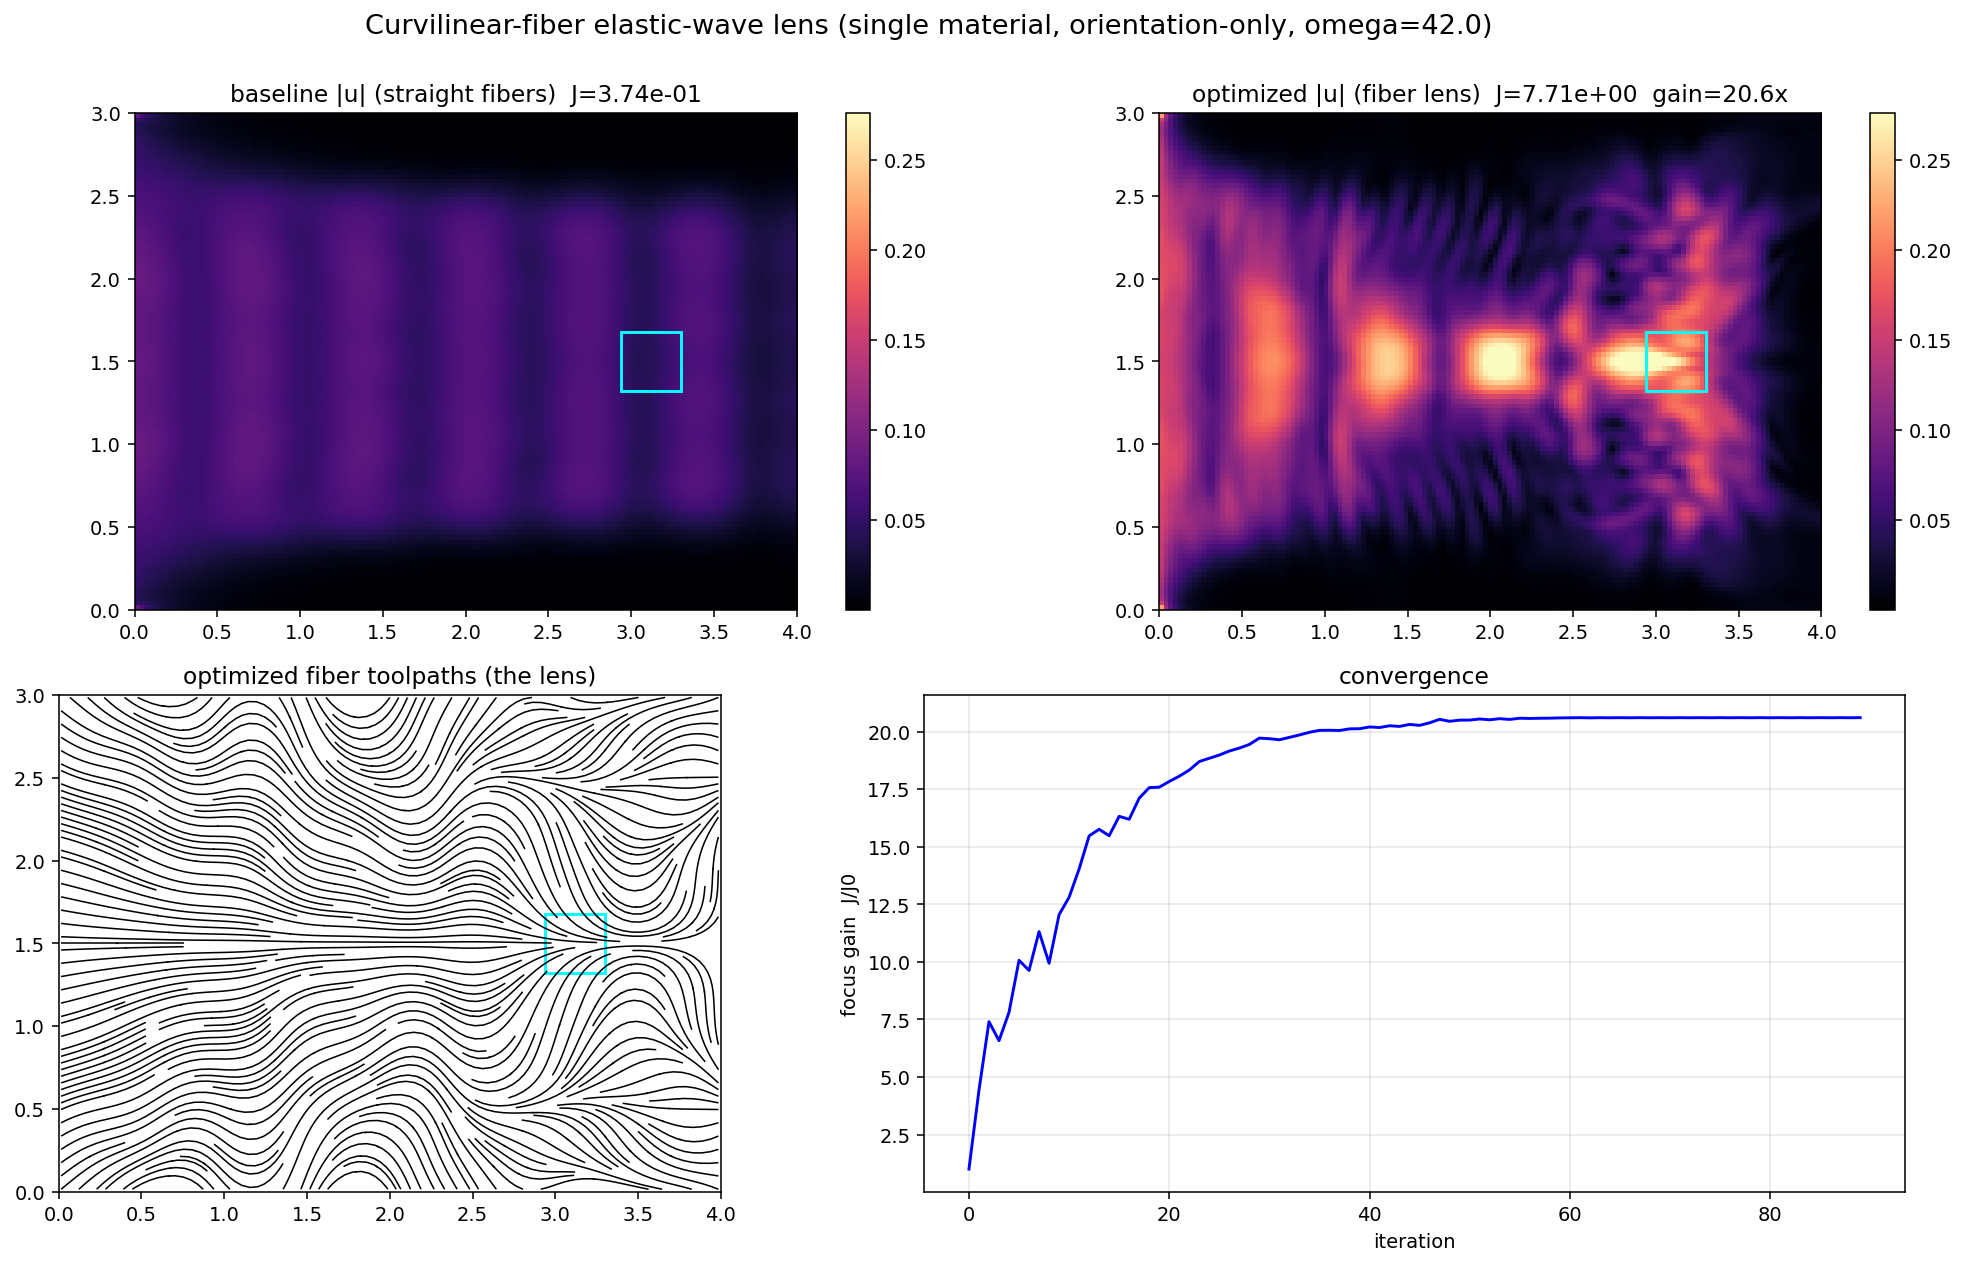
\includegraphics[width=0.84\textwidth]{figs/lens_single.png}
\caption{Curvilinear-fiber wave lens (single frequency, orientation-only):
baseline vs.\ optimized field magnitude, the optimized fiber toolpaths (the
lens), and convergence of the focus gain to $20.6\times$.}
\label{fig:lens}
\end{figure}

\subsection{Broadband localization (multi-frequency)}
A lens optimized for a single frequency is narrow-band: optimizing only the
centre frequency $\omega=38$ yields a $49\times$ gain there but \emph{degrades}
the low frequency below the straight-fiber baseline ($0.55\times$ at $\omega=28$).
Optimizing the worst-case gain \eqref{eq:softmin} over $\{28,38,48\}$ instead
produces a single fiber design that focuses \emph{every} frequency almost
equally, with gains $\{13.8,13.9,13.8\}\times$ (Figure~\ref{fig:multi}). The
max--min objective trades peak single-frequency performance for uniform broadband
performance.

\begin{figure}[h]
\centering
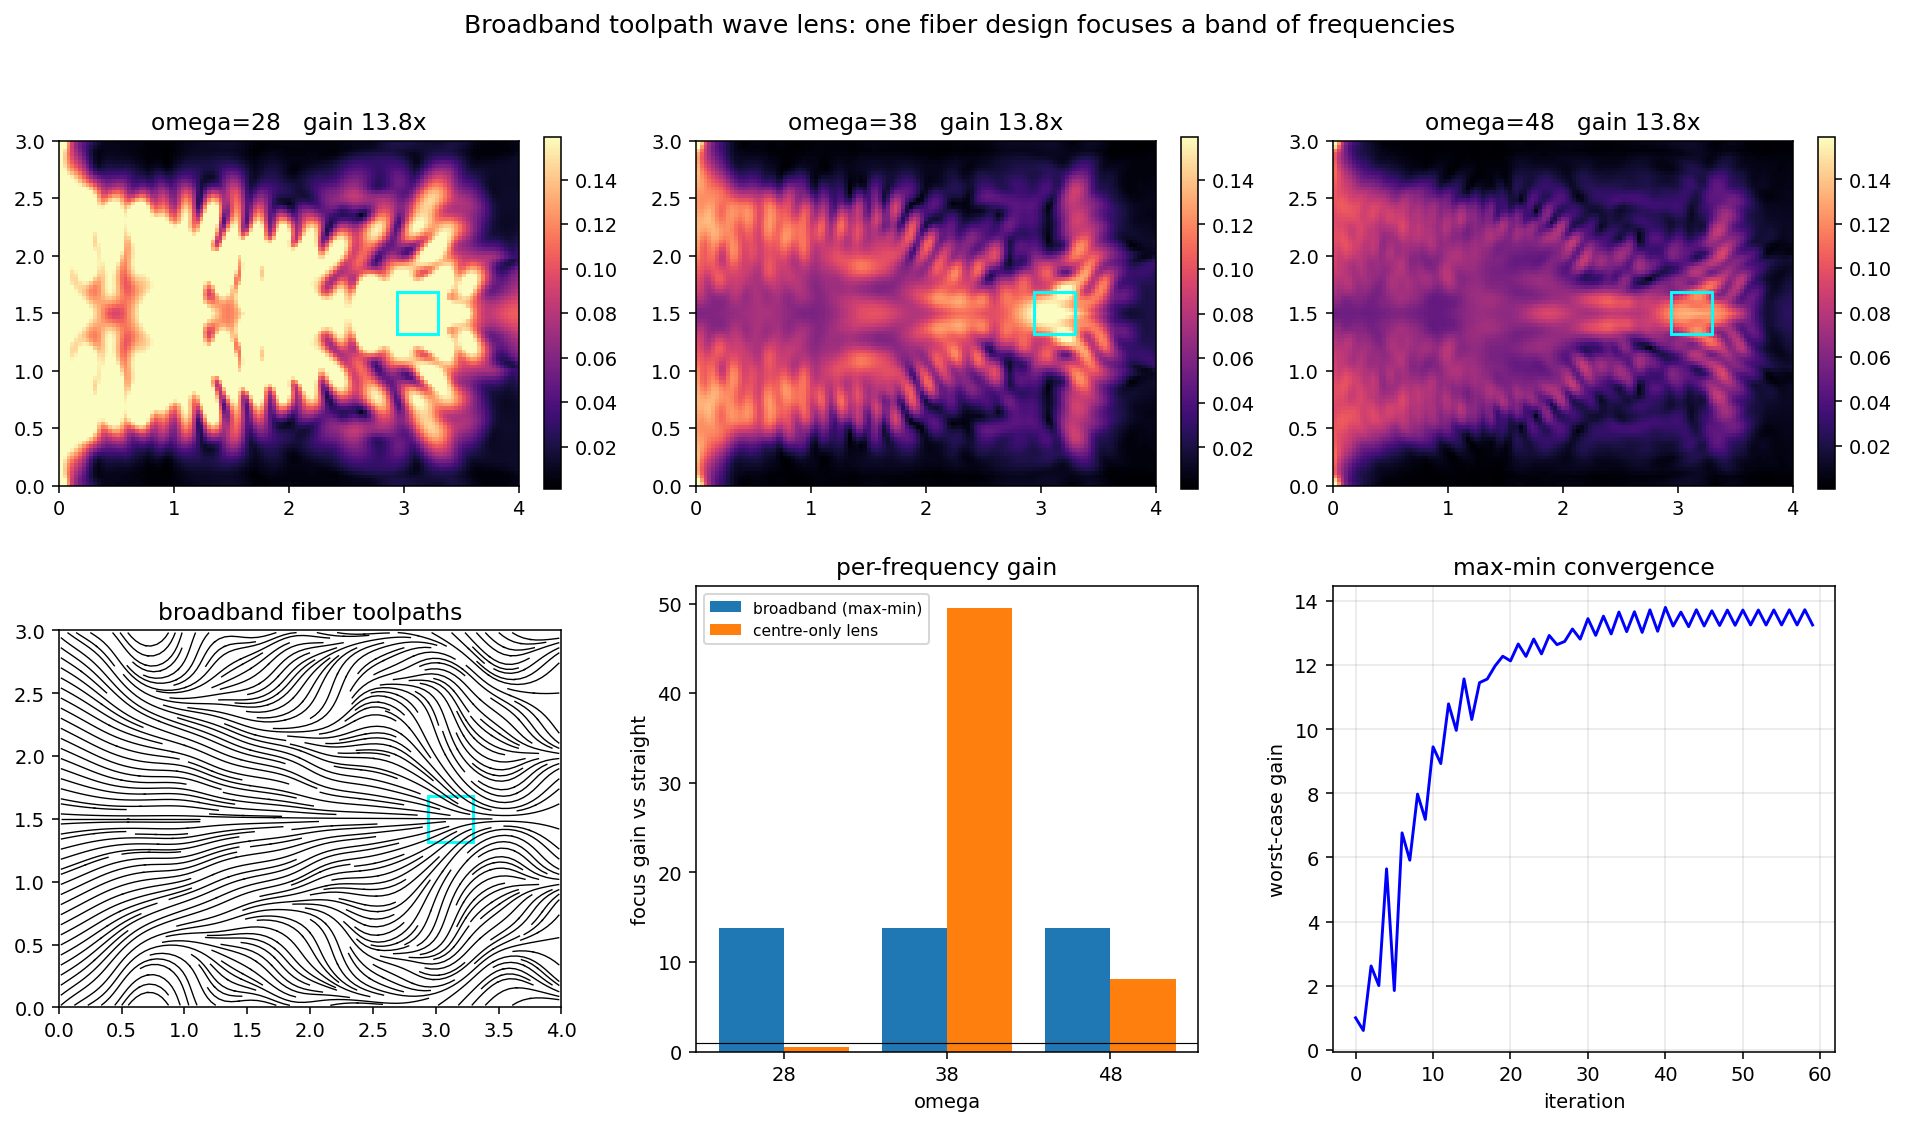
\includegraphics[width=0.92\textwidth]{figs/lens_multi.png}
\caption{Broadband toolpath lens. Top: optimized field at three frequencies, each
focused at the target. Bottom: toolpaths; per-frequency gain of the broadband
(max--min) design vs.\ a narrow-band centre-only lens (which drops below unity at
$\omega=28$); and the worst-case-gain convergence.}
\label{fig:multi}
\end{figure}

\subsection{Elastic cloaking of a void}
A fixed circular void scatters an incident plane wave, casting a downstream
shadow and upstream reflections. Optimizing the fiber orientation in an annular
shell to match the void-free reference reduces the observation-region scattering
energy by $\mathbf{15.3\times}$ (Figure~\ref{fig:cloak}): the shadow is largely
refilled and the reflections suppressed, with the toolpaths visibly wrapping the
void. As expected for orientation-only control of a hard scatterer, a residual
disturbance remains adjacent to the void, but the far field is substantially
restored.

\begin{figure}[h]
\centering
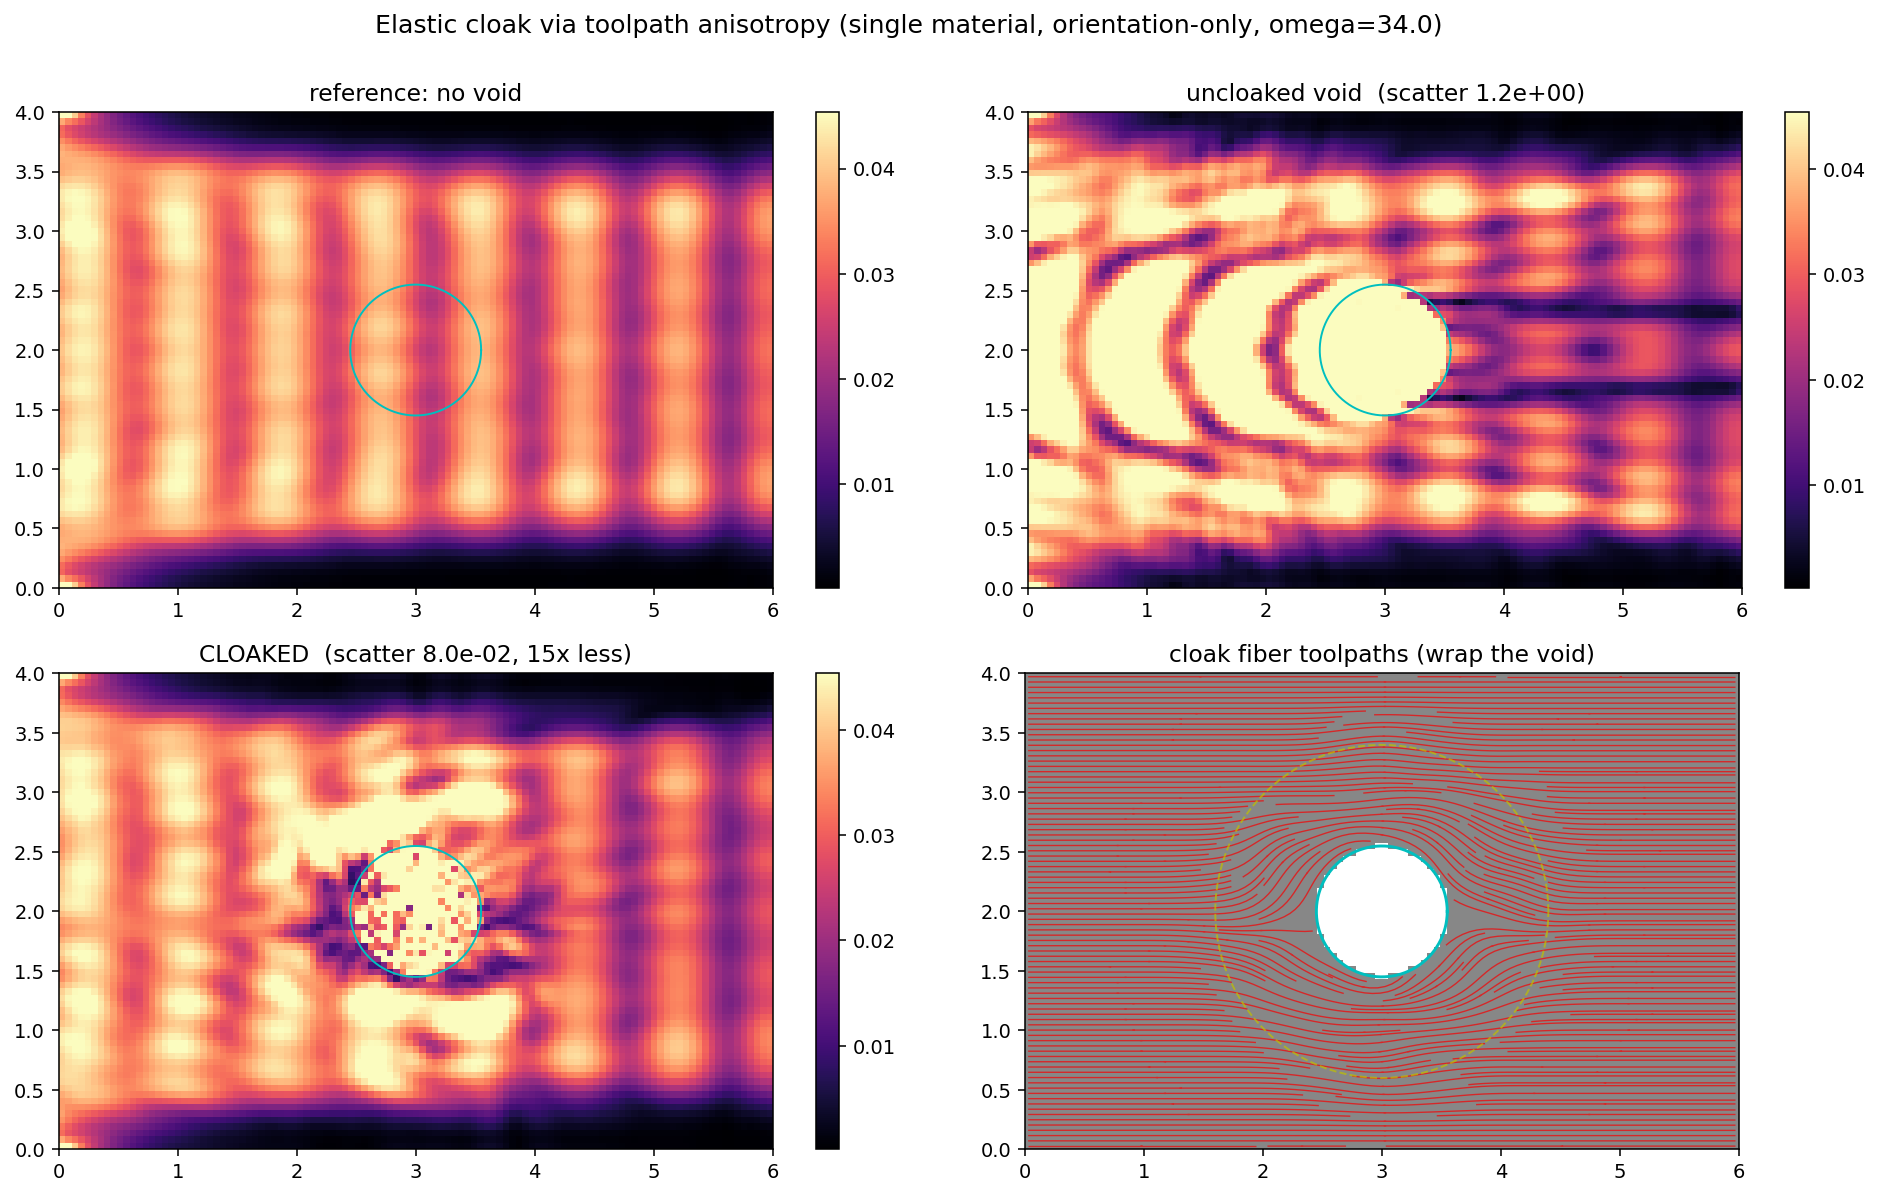
\includegraphics[width=0.88\textwidth]{figs/cloak.png}
\caption{Elastic cloak via toolpath anisotropy: reference (no void), uncloaked
void (strong shadow/reflection), cloaked design ($15.3\times$ less scatter), and
the fiber toolpaths that wrap the void.}
\label{fig:cloak}
\end{figure}

\subsection{Topological valley-Hall waveguide (orientation as the Dirac mass)}
\label{sec:valley}
The same orientation-as-design principle extends to \emph{topological} wave
guiding on periodic cells. We use the scalar (antiplane-shear) problem on a
triangular lattice (lattice vectors $\mathbf a_1=a(1,0)$, $\mathbf a_2=a
(\tfrac12,\tfrac{\sqrt3}{2})$; inequivalent BZ corners $K=(2\mathbf b_1+\mathbf
b_2)/3$, $K'=(\mathbf b_1+2\mathbf b_2)/3$) with a single stiff, C$_{3\mathrm v}$
equilateral-triangle inclusion per cell whose rotation angle $\alpha$ is the
design variable.

\paragraph{$k\!\cdot\!p$ theory.}
When the triangle's mirror planes align with the lattice's ($\alpha\equiv30^\circ$
in our vertex convention) the crystal is C$_{3\mathrm v}$ at $K$ and the second
and third bands meet in a symmetry-protected, \emph{isolated} Dirac cone. Near
$K$ the two-band effective Hamiltonian is
\begin{equation}
  H(\delta\mathbf k)=v_D(\delta k_x\sigma_x+\delta k_y\sigma_y)+m\,\sigma_z,
  \qquad m(\alpha)\propto\cos(3\alpha),
  \label{eq:kp}
\end{equation}
so rotating the triangle away from $\alpha=30^\circ$ breaks the mirror
(C$_{3\mathrm v}\!\to\!$C$_3$) and opens the valley gap $2|m|$, with $m$ changing
sign across $\alpha=30^\circ$. The gapped Dirac cone carries Berry curvature
$\Omega(\delta\mathbf k)=\mp v_D^2 m/2(v_D^2|\delta\mathbf k|^2+m^2)^{3/2}$
concentrated at the valley, giving the quantized \emph{valley Chern number}
$C_v^{K}=\tfrac12\operatorname{sgn}(m)$ and $C_v^{K'}=-\tfrac12\operatorname
{sgn}(m)$ (total Chern zero, as required by time-reversal symmetry). Two domains
with opposite mass (mirror-partner angles $\alpha$ and $60^\circ-\alpha$, e.g.\
$15^\circ$ and $45^\circ$) differ by $|\Delta C_v|=1$, so by bulk--edge
correspondence their interface hosts one gap-traversing, valley-momentum-locked
kink mode per valley.

\paragraph{Design and phase diagram.}
Cells are meshed with periodic, geometry-conforming, unstructured (gmsh)
triangulations --- essential, because a structured/sheared mesh systematically
breaks C$_3$ and splits the Dirac cone at a rate that does \emph{not} vanish
under refinement. Bands are computed with the Bloch reduction \eqref{eq:bloch}.
The rod is sized ($R=0.44a$) and stiffened ($\mu_f/\mu_m=100$) so that the
valley pair is isolated (a full gap of $0.60$ opens on either side of the Dirac
point) with mid-gap frequency $\omega\!\approx\!7.3$. Figure~\ref{fig:vphase}
is the resulting topological phase diagram: the complete valley gap closes
exactly at the Dirac point $\alpha=30^\circ$ (the phase boundary) and is
maximized away from it --- rod orientation is the tunable, optimizable
topological mass.

\paragraph{Gradient optimization of the gap, and an honest accounting.}
The gap is not merely swept but \emph{optimized}. Treating the element density
$\mathbf z$ (geometry) and the fiber-orientation field $\bm\theta$ (anisotropy)
as filtered design fields on the cell, we maximize the complete valley gap
\begin{equation}
  \max_{\mathbf z,\bm\theta}\ \Bigl[\softmin_{\mathbf k\in\mathcal S}\,
  \omega_{p+1}(\mathbf k)-\softmax_{\mathbf k\in\mathcal S}\,\omega_{p}
  (\mathbf k)\Bigr]-c_v(\text{vol}-\text{vol}_\star)^2,
  \label{eq:valopt}
\end{equation}
over a Brillouin-zone sample $\mathcal S$, at fixed volume, by MMA driven by the
Hellmann--Feynman sensitivities $\partial\omega/\partial\mathbf z$ and
$\partial\omega/\partial\bm\theta$ of \eqref{eq:hf} (extended to the P$_1$
triangular mesh and finite-difference verified to $\sim\!10^{-5}$). Running
\eqref{eq:valopt} with the orientation field alone, the density field alone, and
both, isolates the mechanisms (Figure~\ref{fig:vopt}). The result is a genuine
and honest accounting: starting from a seed cell with no complete gap
($-0.54$), optimizing the \emph{orientation} (anisotropy) alone reaches only
$-0.08$ and optimizing the \emph{density} (geometry) alone reaches only $-0.03$
--- \emph{neither field alone opens a complete gap at fixed volume} --- whereas
co-optimizing both opens it ($+0.28$). In this anisotropic-fiber medium the two
levers are complementary: the fiber orientation is a genuine, necessary
ingredient of the optimized topological gap, not a passive accessory. (For an
\emph{isotropic} scatterer, geometry alone suffices, as the phase diagram
above shows; anisotropy becomes essential precisely when the medium is the
fiber composite of interest here.)

\begin{figure}[h]
\centering
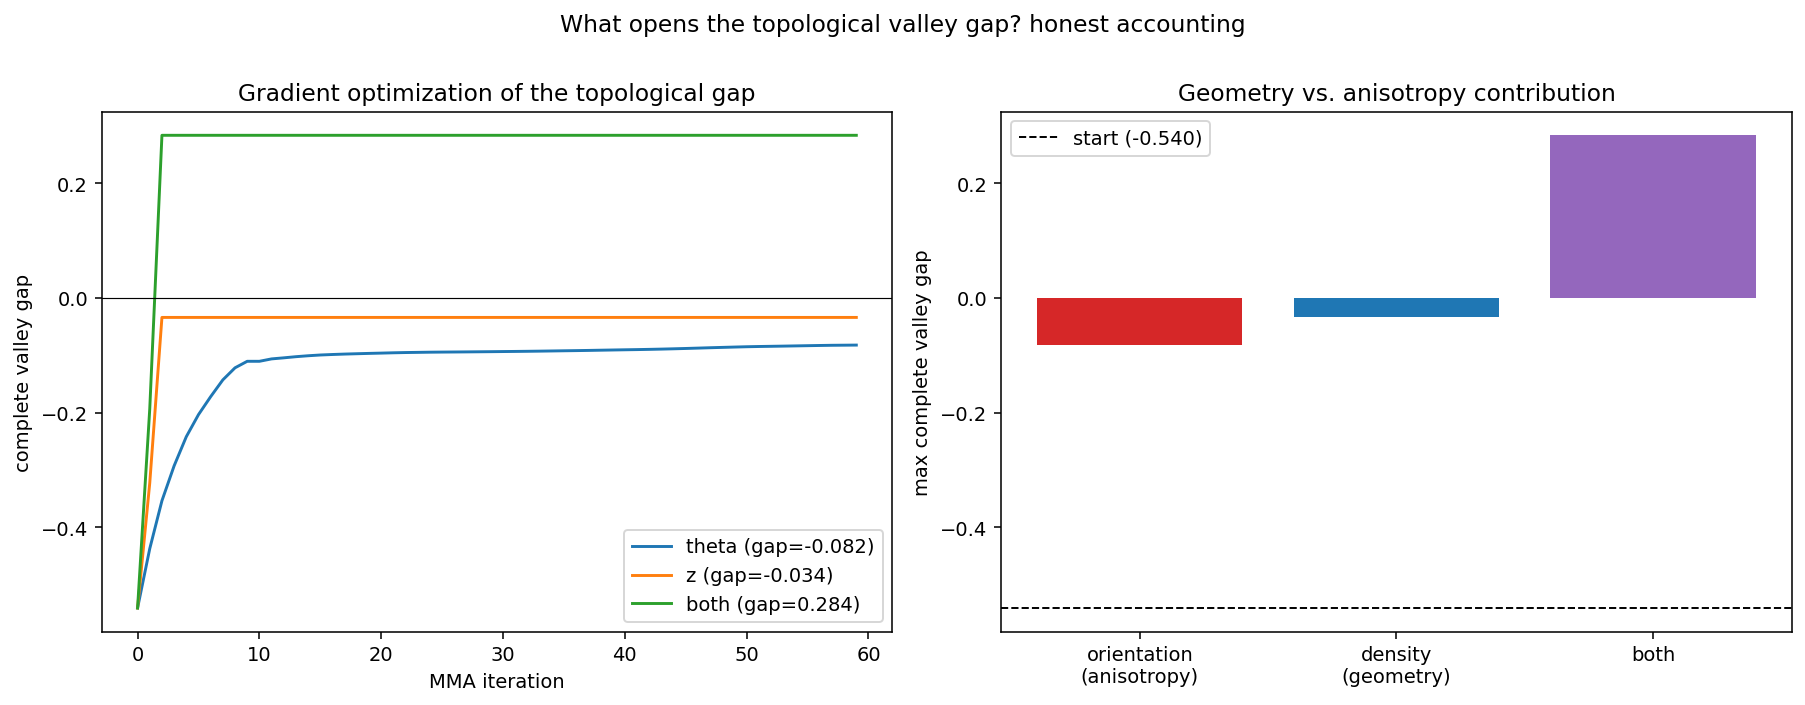
\includegraphics[width=0.92\textwidth]{figs/valley_optimize.png}
\caption{Gradient optimization of the topological valley gap \eqref{eq:valopt} by
MMA + Hellmann--Feynman sensitivities. Left: best-feasible complete gap vs.\
iteration. Right: at fixed volume, orientation-only (anisotropy) and
density-only (geometry) each fail to open a complete gap; only co-optimizing
both succeeds --- an honest measure of the anisotropy's necessary contribution.}
\label{fig:vopt}
\end{figure}

\paragraph{Kink modes and guiding.}
A ribbon supercell with an $\alpha\!=\!15^\circ\,|\,45^\circ$ mirror-partner wall
exhibits a single, strongly wall-localized branch that traverses the entire bulk
gap, connecting the lower and upper bulk bands through the projected valleys
$\kappa=k\!\cdot\!\mathbf a_2=\pm2\pi/3$ (Figure~\ref{fig:vkink}) --- the direct
realization of the bulk--edge correspondence. In a finite domain
(Figure~\ref{fig:vguide}), a time-harmonic source on a domain wall aligned with
the lattice zigzag ($\mathbf a_2$) launches this kink mode: at mid-gap the field
is tightly confined to the wall and transported to the far end, whereas at a
bulk-band frequency it disperses. The wall carries a clean, broadband guided band
across the \emph{entire} bulk gap (transmitted energy $\sim\!10^{1}$--$10^{2}$),
a factor $\sim\!1500$ above the same source at an in-band frequency and
$\sim\!10^{6}$ above the deep-gap (fully reflected) level --- the signature of a
protected edge channel rather than a resonant defect line.

\paragraph{Scope.}
Two honest limitations frame this result. First, a passive elastic medium is
time-reversal symmetric, so only valley-Hall (not chiral quantum-Hall) transport
is available without active components. Second, while straight-wall guiding is
robust and broadband, we found that transmission around a \emph{sharp} $120^\circ$
bend is strongly reduced in this scalar model (the valley polarization, though
sufficient to bind and guide the mode, is not strong enough to fully suppress
inter-valley backscattering at an abrupt corner); high-fidelity cornering would
require further tuning of the rod for maximal valley polarization. The essential
point stands: an \emph{orientation} degree of freedom --- the same design lever
used for the finite-domain devices, and directly analogous to a fiber toolpath
angle --- realizes a tunable topological mass and a working topological edge
waveguide.

\begin{figure}[h]
\centering
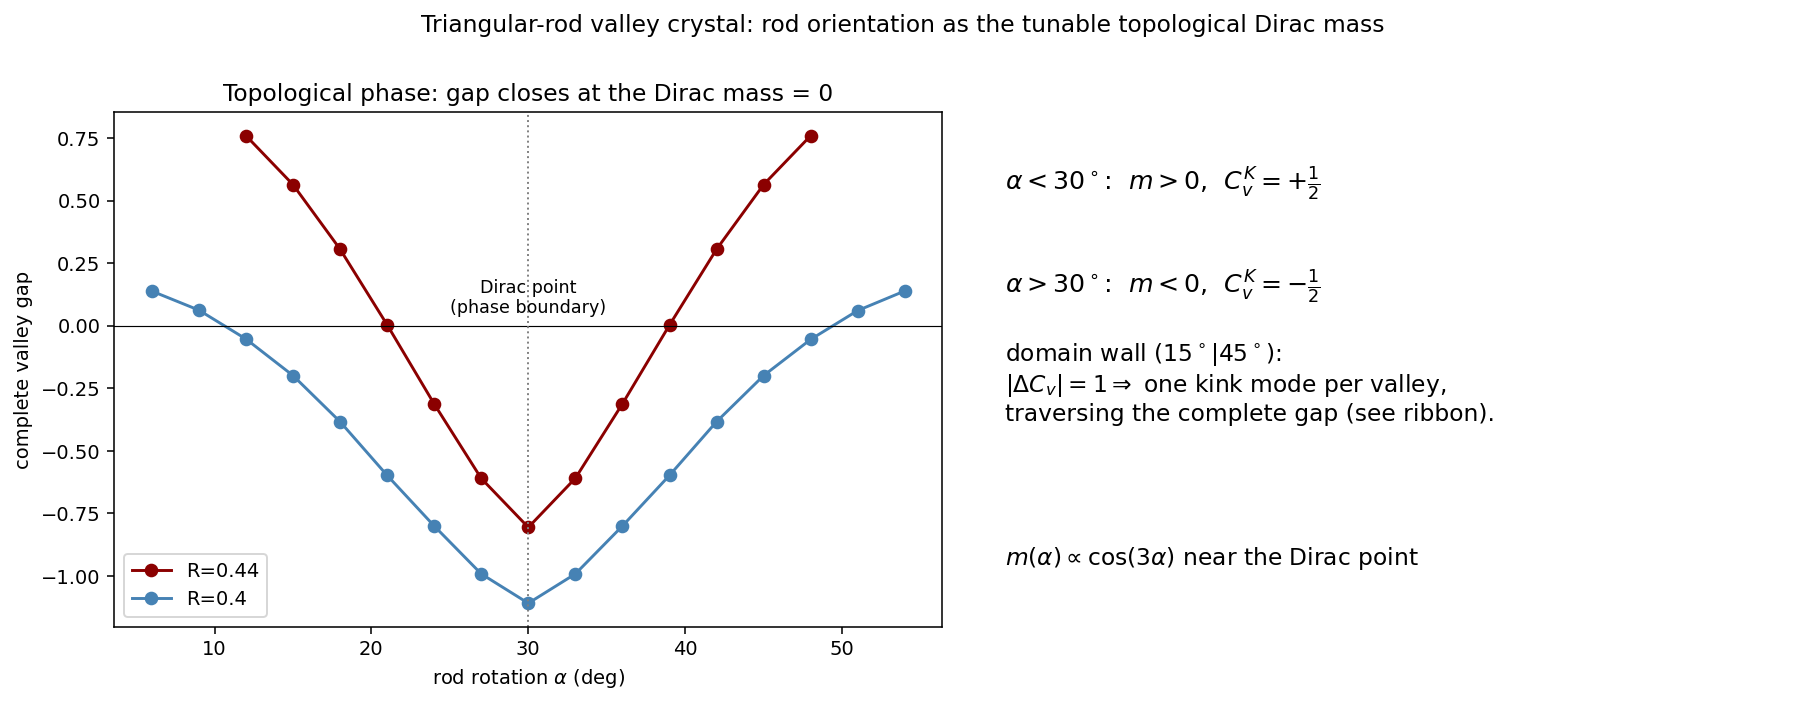
\includegraphics[width=0.92\textwidth]{figs/valley_phase.png}
\caption{Topological phase diagram of the triangular-rod valley crystal: the
complete valley gap (left) closes at the C$_{3\mathrm v}$ Dirac point
$\alpha=30^\circ$ (mass $m=0$, phase boundary) and reopens with opposite valley
Chern on either side. Rod orientation $\alpha$ is the tunable, optimizable
topological Dirac mass; $R$ is the rod size.}
\label{fig:vphase}
\end{figure}

\begin{figure}[h]
\centering
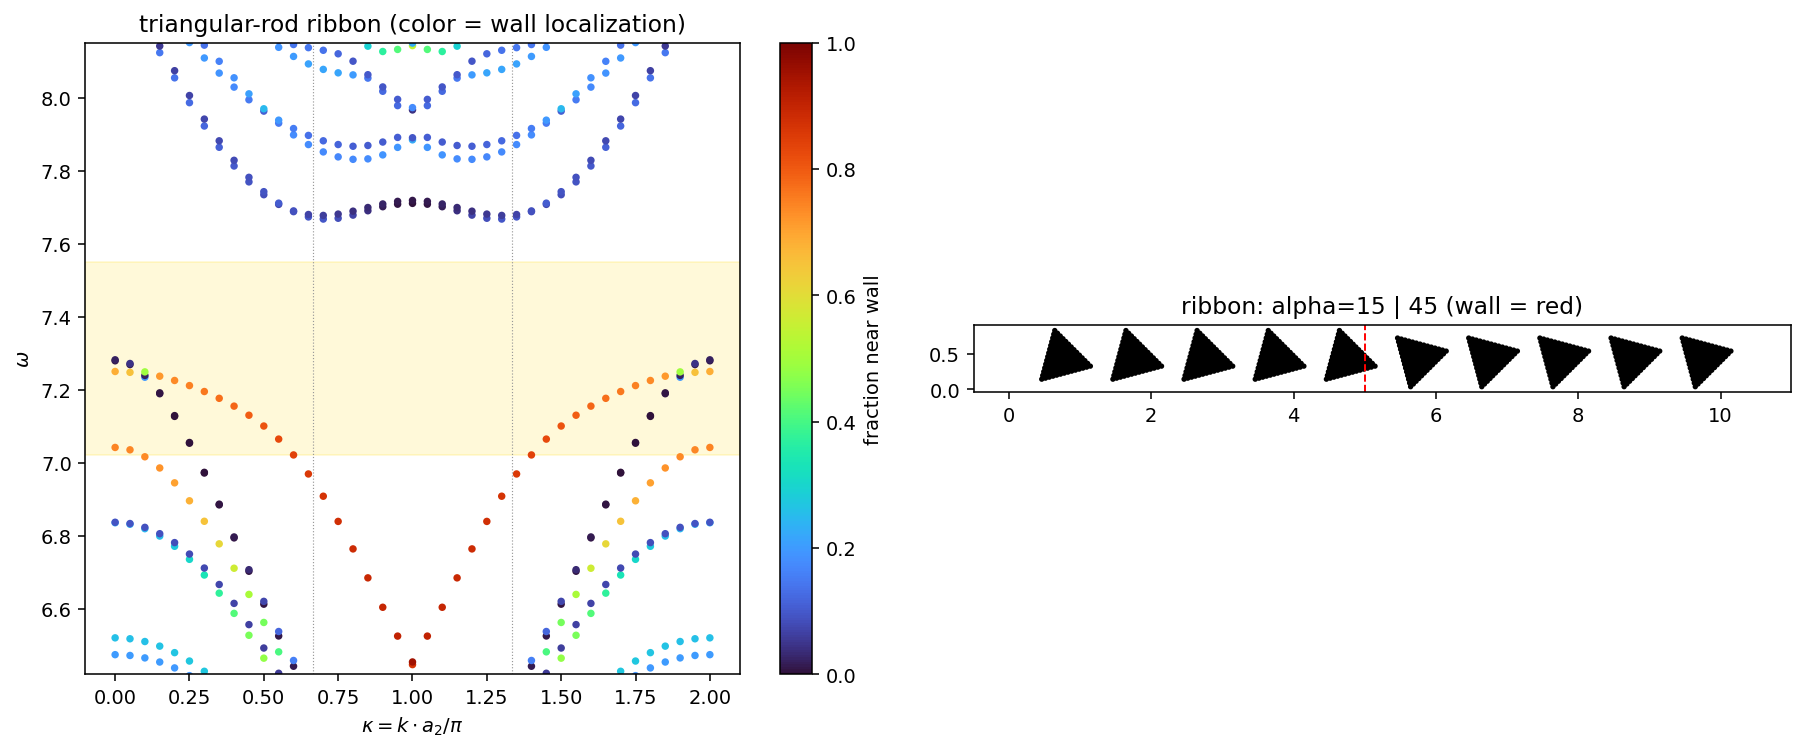
\includegraphics[width=0.92\textwidth]{figs/valley_kink.png}
\caption{Ribbon band structure (left) of an $\alpha=15^\circ|45^\circ$
mirror-partner domain wall (right). A strongly wall-localized (colour = fraction
of modal energy at the wall) branch \emph{traverses} the complete bulk gap
(shaded) through the projected valleys $\kappa=2\pi/3,\,4\pi/3$: the topological
kink mode.}
\label{fig:vkink}
\end{figure}

\begin{figure}[h]
\centering
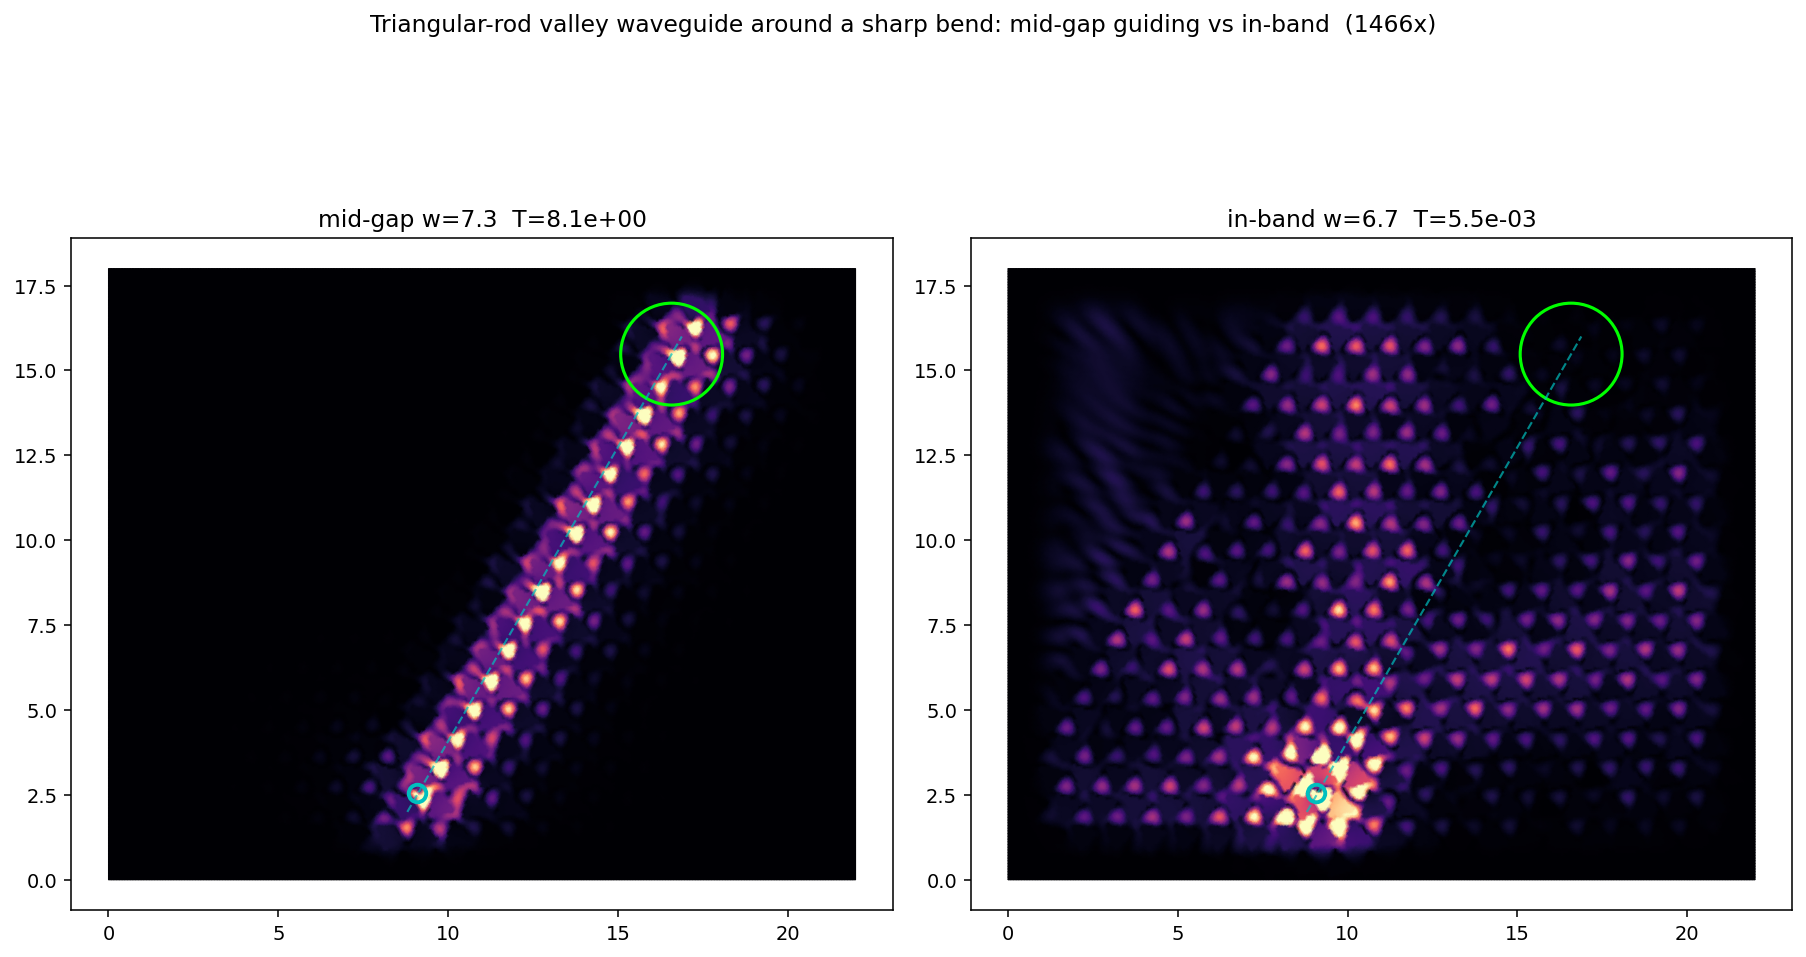
\includegraphics[width=0.92\textwidth]{figs/valley_guide.png}
\caption{Finite-domain valley waveguide. At mid-gap (left) the kink mode is
tightly confined to the lattice-aligned domain wall and transported from source
(cyan) to the output (green); at a bulk-band frequency (right) energy disperses
into the bulk. The mid-gap/in-band transmission ratio is $\sim\!1.5\times10^3$.}
\label{fig:vguide}
\end{figure}

\section{Verification}
Every gradient in this framework is checked against central finite differences,
$\partial_k f\approx[f(\vx{+}\epsilon\mathbf e_k)-f(\vx{-}\epsilon\mathbf e_k)]/
(2\epsilon)$, $\epsilon=10^{-6}$. Table~\ref{tab:verify} collects the worst-case
relative errors, all at or below the finite-difference truncation floor.

\begin{table}[h]
\centering
\caption{Adjoint/Hellmann--Feynman gradients vs.\ central finite differences.}
\label{tab:verify}
\begin{tabular}{lll}
\toprule
Routine & Quantity & max.\ rel.\ error\\
\midrule
Fourier stiffness \eqref{eq:dkf} & $\rmd\mathbf{k}_f/\rmd\theta$ & $8\times10^{-11}$\\
CS-RBF derivatives \eqref{eq:Phix} & $\vPhi_{,x},\vPhi_{,y}$ & $5\times10^{-10}$\\
Wave projection \eqref{eq:wpadj2} & $\partial\hat\chi/\partial(z,\theta)$ & $\sim10^{-6}$\\
Compliance (\S7) & $\partial f/\partial(\vz,\vthh)$ & $\sim10^{-6}$\\
Curl Jacobian \eqref{eq:curljac} & $\partial\zeta/\partial\vthh$ & $1\times10^{-11}$\\
Focus energy \eqref{eq:harmadj} & $\partial E/\partial\vthh$ & $6\times10^{-7}$\\
Multi-frequency \eqref{eq:softmin} & $\partial_{\vthh}$ (sum / minmax) & $6\times10^{-8}/2\times10^{-7}$\\
Cloak (\S11.3) & $\partial J/\partial\vthh$ & $4\times10^{-8}$\\
Eigenvalue \eqref{eq:hf} & $\partial\omega/\partial(\vz,\vthh)$ & $\sim10^{-6}$\\
Berry curvature \eqref{eq:fhs} & Chern (QWZ model) & exact $\{0,\pm1\}$\\
\bottomrule
\end{tabular}
\end{table}

\section{Conclusion}
We have given a complete mathematical and algorithmic description of a unified
density-plus-orientation optimization framework for continuous-fiber composites,
spanning quasi-static curvature-constrained design and time-harmonic wave
control. The exact finite-Fourier representation of the rotated fiber stiffness,
the $C^1$ CS-RBF orientation map with analytic curl, the wave-projection toolpath
operator with its discrete adjoint, and the complex-symmetric harmonic adjoint
together make orientation an inexpensive, fully differentiable design field. In
the finite-domain wave setting, curvilinear fiber toolpaths alone --- with a
homogeneous base material --- focus elastic energy ($>\!20\times$), do so across a
band of frequencies through a max--min objective ($\sim\!14\times$ uniform), and
cloak a void ($\sim\!15\times$ scatter reduction), all driven by adjoint gradients
verified to $\sim\!10^{-7}$. In the periodic setting, the orientation of a
C$_3$-symmetric scatterer acts as a tunable topological Dirac mass whose sign
sets the valley Chern number; a mirror-partner domain wall then guides a
gap-traversing valley-Hall kink mode, realizing a working topological edge
waveguide (mid-gap/in-band transmission ratio $\sim\!10^3$) with the same
orientation lever used for the finite-domain devices. Robust guiding requires an
isolated Dirac cone and a complete gap --- achieved here with a C$_3$-conforming
unstructured mesh and a near-rigid triangular scatterer --- and, for sharp
$120^\circ$ corners, strong valley polarization that remains a design target. The
manufacturability machinery carries over unchanged, making these designs
candidates for additive fabrication.

\begin{thebibliography}{9}
\bibitem{wong2026} J.~Wong, E.~D.~Sanders, D.~W.~Rosen,
  \emph{Toolpath-integrated topology optimization for design of additively
  manufactured fiber-reinforced structures considering limits on fiber
  curvature}, Composite Structures \textbf{378} (2026) 119897.
\bibitem{wong2025} J.~Wong, E.~D.~Sanders, D.~W.~Rosen,
  \emph{Topology optimization of additively manufactured continuous
  fiber-reinforced structures with constraints on fiber path geometry},
  Struct.\ Multidiscip.\ Optim.\ \textbf{68} (2025).
\bibitem{ren2024} H.~Ren, D.~Wang, G.~Liu, D.~W.~Rosen, Y.~Xiong,
  \emph{Concurrent optimization of structural topology and toolpath for additive
  manufacturing of continuous fiber-reinforced polymer composites}, Comput.\
  Methods Appl.\ Mech.\ Engrg.\ \textbf{430} (2024) 117227.
\bibitem{wendland1995} H.~Wendland,
  \emph{Piecewise polynomial, positive definite and compactly supported radial
  functions of minimal degree}, Adv.\ Comput.\ Math.\ \textbf{4} (1995) 389--396.
\bibitem{senhora2020} F.~V.~Senhora, O.~Giraldo-Londo\~no, I.~F.~M.~Menezes,
  G.~H.~Paulino, \emph{Topology optimization with local stress constraints: a
  stress aggregation-free approach}, Struct.\ Multidiscip.\ Optim.\ \textbf{62}
  (2020) 1639--1668.
\bibitem{svanberg1987} K.~Svanberg,
  \emph{The method of moving asymptotes---a new method for structural
  optimization}, Int.\ J.\ Numer.\ Meth.\ Engng.\ \textbf{24} (1987) 359--373.
\bibitem{fukui2005} T.~Fukui, Y.~Hatsugai, H.~Suzuki,
  \emph{Chern numbers in discretized Brillouin zone: efficient method of
  computing (spin) Hall conductances}, J.\ Phys.\ Soc.\ Jpn.\ \textbf{74} (2005)
  1674--1677.
\end{thebibliography}

\end{document}
